%!TeX root=../tese.tex
%("dica" para o editor de texto: este arquivo é parte de um documento maior)
% para saber mais: https://tex.stackexchange.com/q/78101/183146

% Os capítulos de compõem a dissertação/tese, com numeração normal, podem
% ser inseridos diretamente aqui ou "puxados" de outros arquivos.
% Em alguns (raros) casos, pode ser interessante usar \include ao
% invés de \input: https://tex.stackexchange.com/a/32058/183146
%!TeX root=../tese.tex
%("dica" para o editor de texto: este arquivo é parte de um documento maior)
% para saber mais: https://tex.stackexchange.com/q/78101/183146

%% ------------------------------------------------------------------------- %%
\chapter{Introduction}
\label{cap:introduction}

% Colocar uma prévia do trabalho em si, não só do contexto

Social networks have all but taken over contemporary daily life. From the
eponymous socializing, to reading news, to expressing ourselves, social media
has creeped into every corner of society. Most of its side-effects, it could be
argued, are positive (shortening distances, political accountability, social
organizing), but they are not perfect institutions.

Social media companies already face significant backlash for their questionable
business model and ethics. Cambridge Analytica's election meddling \citep{}, % Revealed: 50 million Facebook profiles harvested for Cambridge Analytica in major data breach
Facebook's subliminal experiments \citep{}, YouTube's problem with disturbing % Experimental evidence of massive-scale emotional contagion through social networks
content marketed at kids \citep{}, and Twitter's bot infestation \citep{} are % YouTube's latest hit: neon superheroes, giant ducks and plenty of lycra % Online Human-Bot Interactions: Detection, Estimation, and Characterization
just a few recent scandals that have put the societal role of social media into
question.

One particular controversy that has taken over public discourse around social
networks is the role that their algorithms might have in radicalizing users,
specially younger ones. The aforementioned experiments conducted by Facebook to
influence people's emotions and the proliferation of more than questionable
videos aimed at children on YouTube are instances that seem to corroborate the
notion that there is something fundamentally wrong with these companies'
algorithms.

News organizations, in general, have been skeptical of social networks.
Journalists and specialists alike argue that social media's algorithms
(specially recommender algorithms) are tuned to peddle conspiracy theories,
extremist views, and false information \citep{}. This would be the source cause % Mozilla Explains: Why Does YouTube Recommend Conspiracy Theory Videos?
for a plethora of what they consider contemporary evils: religious extremism,
anti-democratic leaders, widespread depression among teenagers, anti-science
movements, etc.

This narrative, of course, has been questioned for a variety of reasons. Some
say that it is self serving: traditional news organizations are being displaced
by social media and it would be convenient for them to mine the public's trust
in them \citep{munger_right-wing_2020}. Others claim that these recommender
algorithms are not to blame for political polarization and that social networks
even have a tendency to favor more left-wing viewpoints
\citep{ledwich_algorithmic_2019}.

The debate around the role of recommender systems in social media radicalization
is still, unfortunately, too recent and based in anecdotes. Since its impacts
are all but universal, more quality research is vital to inform both the public
and opinion makers about if and how much recommendation algorithms influence
social media users.

This dissertation aims to further such research.

\section{Social Networks}
\label{sec:social_networks}

Social networking services, also referred to as social networks and social
media, are notoriously difficult to define. Some definitions might be too narrow
(excluding instant messaging services), while some might be too broad (including
technologies such as telephone networks). Most definitions \citep{} include some % Social Network Sites: Definition, History, and Scholarship
common features:

\begin{itemize}
  \item Internet-based
  \item Focus on user-generated content
  \item Users have profiles
  \item Users can connect
\end{itemize}

While social-networking-like applications already existed in Usenet, Geocities,
launched in 1994, is usually regarded as the first major social network.
Friendster and Myspace followed in 2003, with Orkut and Facebook slightly
lagging behind in 2004. Each hit their peak at different moments and different
countries, but Facebook overtook all of them in 2009 when it became the most
popular social networking service in the world, still maintaining the title over
13 years latter at the moment of writing \citep{}. % Biggest social media platforms 2022

Even though all aforementioned social networks are multimedia, that is, users
can post text, photos and videos, some of the most popular services focus on a
specific type of media. For instance, YouTube (2009) centers around videos,
WhatsApp (2009) and WeChat (2011) were originally designed for text-based
communication, and Instagram's (2010) main focus is photos.

Parallel to all other features and idiosyncrasies, there lay the recommendation
algorithms. While a few social networking services (e.g. WhatsApp) do not
recommend any content or profiles to the user, most do and, according to recent
studies, these recommendations have become the main drivers of interactions
\citep{}. % acho que é um da stoica

\section{Recommender Systems}
\label{sec:recommender_systems}

Recommender systems (sometimes called recommendation systems or recommender
algorithms) first appeared in 1992 under the name ``collaborative filtering'',
even though that term nowadays refers to a subclass of recommender systems
\citep{goldberg_using_1992}. The aim of such an algorithm is providing users
with personalized product or service recommendations, an essential task when
considering the ever increasing number of possible videos to watch, music to
listen, products to buy.

The input of a recommender system is usually information about the preferences
(ratings, likes/dislikes, watch time, etc.) of consumers for a set of items.
Preference information can be gathered from explicit behaviors (e.g. rating a
product in a scale ranging from 0 to 5 stars) or from implicit behaviors (e.g.
how much time the user lingers on a product's page). These data can be combined
with information about the user (age, political leaning, etc.) in order to
create the best possible representation of the user's preferences.

The output of these systems can come in the form of a prediction or a list of
recommended items. In the first case, the goal of the algorithm is approximating
the rating a user would attribute to a yet unrated item, while the second type
of output involves gathering the items that most likely would interest the user.
Simple recommender systems that suggest items similar to the one being queried
do not necessarily involve rating predictions, but it is common to have the list
of recommended items based on the ratings the algorithms estimated the user
would give to those items.

Most recommender systems fall into one of four categories according to the
filtering algorithm they use, that it, the strategy for generating predictions
or selecting the top-N items: content-based filtering, demographic filtering,
collaborative filtering, and hybrid filtering
\citep{bobadilla_recommender_2013}.

Content-based filtering leverages characteristics of the content in order to
generate the recommendations \citep{ricci_introduction_2011}. One such algorithm
might use the genres of watched movies in order to recommend new ones, while
another might analyze the sound signature of a song to recommend similar ones,
but, either way, all content-based systems establish a similarity between items
as a basis for recommendations. Analogously, demographic filtering uses
demographic data to establish a similarity between users and recommend items
positively rated by similar people.

Collaborative filtering algorithms also recommend items that similar users
liked, but, in this case, the similarity between users is based on past ratings
and not demographic information \citep{ricci_introduction_2011}. Hybrid
filtering usually mix collaborative methods with either content-based or
demographic filtering \citep{ricci_introduction_2011}.

As with other knowledge-based systems, recommendation algorithms have quickly
incorporated neural networks and other machine learning techniques over the past
few years. Even though the implementation of YouTube's recommendation algorithm
is a trade secret, it is known to gather enormous amounts of data about the
user's interaction with the website and to require Google's own TPUs in order to
be trained. It also involves two distinct steps: candidate generation (when the
billions of videos available on the platform are quickly narrowed down to a few
hundreds that might be relevant) and ranking (when the algorithm actually
attempts to predict the score a user would implicitly give to the candidate
videos) \citep{}. % Improving Relevance Prediction with Transfer Learning in Large-scale Retrieval Systems

Another relevant aspect of recommender systems that is well-exemplified by
YouTube is the use of balancing factors such as novelty, dispersity, and
stability \citep{zhao_recommending_2019}. In the case of Google's video giant,
there is a baked-in bias for recency, strongly favoring newer videos in
detriment of older content \citep{zhao_recommending_2019}.

From this kind of bias stems much debate: as recommender systems explode in
popularity, so does research regarding its shortcommings. User radicalization
and algorithmic bias (explicitly programmed or not) are hotly debated subjects
in the literature.

\section{Radicalization and Bias}
\label{sec:radicalization_bias}

Opinion polarization is far from a recent phenomenon, and social media is only
the most recent communication medium where it can be detected and studied. An
important question is whether it facilitates or attenuates polarization:
anecdotal evidence might suggest that social network structures incentivize
users to gather into antagonistic communities, but this could be a result of
people simply being more likely to express their preferences online, not of some
intrinsic property of social media.

One possible byproduct of polarization is radicalization. Despite not being
entirely different phenomena, these concepts deserve distinct levels of
attention. While polarization can be considered a natural part of democratic
discourse, radicalization only happens when certain conditions are met. UNESCO
defines radicalization as \citep{seraphin_youth_2017}:

\begin{itemize}
  \item The individual person's search for fundamental meaning, origin and
        return to a root ideology;
  \item The individual as part of a group's adoption of a violent form of
        expansion of root ideologies and related oppositionist objectives;
  \item The polarization of the social space and the collective construction of
        a threatened ideal 'us' against 'them,' where the others are dehumanized
        by a process of scapegoating.
\end{itemize}

The third point is of special importance to the distinction between polarization
and radicalization. The first might be a simple consequence of democratic
disagreements between opposing parties, but the latter involves a dehumanization
of the opposition, which can lead to extremism: radicalism so intense that the
only effective strategy is physically exterminating the opposition.

Understanding how polarization might lead to radicalization (and, ultimately, to
extremism) is, therefore, of paramount significance to cultivate healthy
democracies, specially in the digital age. Since most social networks, as of
this writing, are still poorly moderated, they allow users to be exposed to a
plethora of viewpoints, from benign to insidious, possibly configuring a
``pipeline of radicalization'' through which regular users end up radicalized by
coming into contact with extreme content \citep{ribeiro_auditing_2020}.

Of course this argument is still very much open for debate. As will be shown in
Chapter~\ref{cap:review}, researchers have found evidences both for and against
the pipeline hypothesis and even proposed other means though which social media
might help radicalize users (e.g. the supply and demand hypothesis
\citep{munger_right-wing_2020}). Despite all disagreements, one common point
addressed by most research is the role of recommendation algorithms in serving
users with radicalizing content.

Proponents of the pipeline hypothesis, for instance, argue that recommendation
systems, aiming to maximize content consumption, suggest items that reinforce
preconceived notions of the user and that play on fear and paranoia
\citep{ribeiro_auditing_2020}. Content that appears urgent and leaves the user
fearful (for their live, their community, or their identity) could be more
engaging and, therefore, might be more susceptible to being considered as
relevant by the algorithm.

Even if the pipeline hypothesis is correct, specifics of how much algorithms are
to blame for radicalization are still unknown and hard to pin down. Most
research about the subject focuses on specific platforms (like Twitter and
YouTube) and have severe limitations with regards to how much data those
companies make available, not to mention the constant changes made to the
algorithms over the years that might alter their radicalization properties.
Definitive evidence for one theory or another must, therefore, apply to
recommender systems in general and be predictive of how they work both in
controlled and real life scenarios.

% mesclar parágrafo abaixo

YouTube, for example, currently has over 2 billion monthly logged-in users
\citep{}, but it makes no significant effort to clarify changes made to the % https://blog.youtube/press/
algorithm or even whether they fulfill their promises of reducing user exposure
to radicalizing content. With more than 500 hours of content being uploaded
every minute \citep{}, if 1\% of all videos can be considered radicalizing and % https://blog.youtube/press/
the algorithm can detect 99\% of them, that still leaves over 25.000 hours of
brand new extremist content free to spread on the platform every year. This goes
to show that, in the scale that these companies operate, even a small fraction
of content might still be enough to influence the overall recommendations made
by the algorithm. It is also worth noting that most of these platforms' efforts
are concentrated in their parent countries (usually the United States), so, even
if they actually try and remove the offending content, most of the
non-English-speaking world would still not be impacted by their policy changes.

Closely related to user radicalization is the subject of algorithmic bias.
YouTube, for example, has an explicit bias towards recency
\citep{covington_deep_2016}, meaning that more recent videos get "boosted" by
their recommendation algorithm. This is explicitly coded into the system, but
there are also implicit biases, learned by watching user behavior.

Stoica \citep{stoica_algorithmic_2018} studied Instagram profiles before and
after the implementation of their recommendation engine. They discovered that
male users had a slight predilection for following other men, while women
displayed no such preference and, as soon as the recommender system was
deployed, engagement with profiles of male users skyrocketed even though they
were the minority on the platform. The algorithm recognized and leveraged this
so called differentiated homophily effectively, but we might question whether or
not this should be the desired outcome of a good recommender system.

In social networks where recommendations are front and center, such as YouTube,
the algorithm could go from being a mere reflection of user preferences to
actively shaping user behavior. Hypothetically, a minoritary group of highly
engaged users with strong self-reinforcing consumption habits could tip the
scales of the algorithm and cause fringe content to be amplified; this is only
one way through which a radicalization pipeline could spontaneously form in a
social network.

% If this stuff happens at a sufficient scale (big % of the web), it could stop generative text models in their tracks -- their performance would degrade as they start training on their own output.

\section{Research Goals}
\label{sec:research_goals}

As explained in the previous sections, social networks' recommendation
algorithms might play a significant role in radicalizing users. This could be,
at least in part, be a result of implicit and explicit biases in recommender
systems.

This dissertation aims to explore the radicalization pipeline hypothesis and,
more specifically, understand the mechanisms through which recommender systems
can end up learning or developing biases. The research developed here revolves
around the dynamical properties of recommender systems (i.e., the sequence of
items suggested to an arbitrary user over time) and how feedback loops can
create ``amplification pipelines'' inside these engines.

In short, the main motivator of this research is to test the pipeline hypothesis
in a setting where recommendation algorithms learn dynamically.

\section{Outline}
\label{sec:outline}

...

\par

%!TeX root=../tese.tex
%("dica" para o editor de texto: este arquivo é parte de um documento maior)
% para saber mais: https://tex.stackexchange.com/q/78101/183146

\chapter{Literature review}
\label{cap:review}

There are three types of work that are relevant to the current topic: general
literature about recommender systems, evidences of algorithmic bias, and methods
of creating fairer recommendations. Since this area of study is still mostly
unexplored, there is no consensus on whether social media recommender systems
favor extremist content (or even whether they are actually deradicalisation
agents), which means that many references used in this work might disagree
amongst themselves.

\section{Scientific literature}
\label{cap:scientific}

General literature about recommendation algorithms is abound. One of the most
cited surveys was elaborated by \citet{bobadilla_recommender_2013}, but
works by \citet{he_interactive_2016} (about interactive recommender systems),
and by \citet{kunaver_diversity_2017} (about diversity in recommender systems)
were also used in order to draw a complete panorama of the field.

Another relevant article, by \citet{guy_social_2010}, is the landmark paper that
inaugurates the usage of user data alongside labels to create a recommendation
algorithm that is highly accurate and a staple of modern social networks. This
essentially starts the usage of recommenders systems in social media.

When talking specifically about YouTube's recommendation algorithms, two papers
deserve special attention. The first one, by \citet{covington_deep_2016}, marks
YouTube's move towards the usage of deep neural networks to generate video
recommendations. The authors describe a two-stage model that first generates a
list of candidates and then ranks them, also reporting dramatic performance
improvements. The second one, by \citet{zhao_recommending_2019}, describing a
more recent version of YouTube's recommendation algorithm, explores the
Multi-gate Mixture-of-Experts technique to optimize recommendations for more
than one ranking objective and the Wide \& Deep framework to mitigate selection
biases. The authors also make it clear that YouTube's recommender system has a
strong bias towards more recent content instead of more traditional metrics.

Many authors have also explored how biases in recommendation engines might lead
to user radicalization. \citet{agarwal_topic-specific_2015} developed an early
example of a technique to try and find extremist content on YouTube. Using
advanced machine learning methods, the authors create a YouTube crawler that
starts from a seed video and iteratively classifies featured channels and videos
according to their potential extremism. A more recent example of this can be
found in \citet{tangherlini_automated_2020}, where the authors propose a novel
approach for identifying conspiracy theories online. By analyzing the narrative
structure of a conspiracy theory (Pizzagate) and comparing it to an actual
conspiracy (Bridgegate), they create a model that can guess whether a
conspiratorial narrative is or not fabricated. According to their findings, a
multi-domain nature and the presence of keystone nodes are signs that strongly
indicate a conspiracy theory.

Besides just finding and identifying radicalizing content on YouTube, many
authors have been concerned with studying the radicalization dynamics directly.
\citet{alfano_technologically_2020}, for example, claim to be ``the first
systematic, pre-registered attempt to establish whether and to what extent the
recommender system tends to promote such [extremist] content.''
\citet{cho_search_2020} also attempt to understand how users can be radicalized
by the algorithm. By experimentally manipulating user search/watch history, the
authors concluded that algorithmically recommended content can reinforce a
participant's political opinions.

In the same vein, \citet{faddoul_longitudinal_2020}, after some high-profile
cases of users being radicalized through YouTube videos, studied the efforts
announced by the platform to curb the spread of conspiracy theories on the
website. The paper aimed to verify this claim by developing both an emulation of
YouTube's recommendation algorithm and a classifier that labeled whether a video
is conspiratorial or not. The authors describe an overall decrease in the number
of conspiracy recommendations, though not when weighing these recommendations by
views.

Three papers that deserve a closer look are those that investigate how regular
recommendation algorithms can learn covert biases in the users of a social
network and amplify them to previously unimaginable rates.
\citet{stoica_algorithmic_2018} explore the existence of an ``algorithmic glass
ceiling'' and introduces the concept of differentiated homophily. The authors
experiment on a Instagram dataset before and after the introduction of
algorithmic recommendations and discover that, even though most of that
network's users were female, the most followed profiles were male. They explain
this phenomenon by postulating that the algorithm learns biases in the
population, that is, male preference for male profiles (which doesn't happens
for females and thus characterizes an asymmetric---differentiated---homophily),
and ends up enhancing this effect. \citet{stoica_hegemony_2019}, building on top
of their previous work, create a proposal for new recommender systems that take
differentiated homophily into account in order to reduce the ``glass ceiling''
effect observed in non-corrected recommendation algorithms. The work focuses on
the theoretical description of the algorithm, but also attempts to validate its
hypothesis in real world data. \citet{stoica_algorithmic_2020}, in their most
recent paper, show that the most commonly used metrics in recommender systems
``exacerbate disparity between different communities'' because they reinforce
homophilic behavior of the network. This has profound implications, since these
algorithms might further suppress already minoritary viewpoints without being
explicitly programmed to do so.

Like the aforementioned articles, \citet{matakos_maximizing_2020} also propose a
novel recommendation algorithm that tries to strike a balance between
information spread and ensuring that the users are exposed to diverse
viewpoints. The authors show that this goal is important if we want to foster
healthy online debate, and that the algorithm is efficient and scalable with a
minor approximation. One possible inspiration for these papers might be one by
\citet{su_effect_2016} that studyed the network structure of Twitter before and
after the introduction of algorithmic recommendations (``Who to Follow''). The
authors of the paper discovered that all users benefitted recommendations, but
that users with already popular profiles benefitted even more, effectively
changing the network structure and dynamics. \citet{caton_fairness_2020} have
recently compiled other valuable information on fairness in machine learning
into a survey.

Because of data limitations, there still are few studies that investigate how
recommendation algorithms work dinamicaly, over time.
\citet{burke_evaluating_2010} point out that most methods for evaluating
recommender systems are static, that is, involve static snapshots of user and
item data. The authors propose a novel evaluation technique that helps provide
insight into the evolution of recommendation behavior: the ``temporal
leave-one-out'' approach. A more recent example of this approach was developed
by \citet{roth_tubes_2020}. Their paper delves into the confinement dynamics
possibly fostered by YouTube's recommendation algorithm. The authors create,
from a diverse set of seed videos, a graph of the videos iteratively recommended
by YouTube and, from this, study whether there were created ``filter bubbles''.
They find that indeed YouTubes recommendations are prone to confinement dynamics
be it topological, topical or temporal.

Even more recently, \citet{yao_measuring_2021} propose an approach for measuring
recommender system bias based on simulated users. Even though this work focuses
only on bias towards popular content, it is of particular importance because it
was written by researchers from Google itself. Some years before,
\citet{dash_network-centric_2019} also proposed a framework for auditing
recommender systems based on its network of users. Another contribution of their
work is a novel quantifications of diversity.

A different approach to understanding biases in recommendation algorithms range
from analyzing similarity metrics to developing theoretical bounded confidence
models. \citet{giller_statistical_2012} goes with the first strategy, and
identifies certain aspects of cosine similarity that are often overlooked.
Starting from simple theorems regarding the density of n-dimensional spheres,
the author concludes that the expected cosine similarity between random
bitstreams might be significantly different from the average. This is noteworthy
because many recommendation algorithms use cosine similarity in order to
determine the similarity between two items to recommend.
\citet{sirbu_algorithmic_2019} go with the latter, providing an interesting
theoretical model of how inherent biases in algorithmic recommendations might
highten opinion polarization. Using a bounded confidence model, the authors
propose the addition of a $\gamma$ term that represents the odds of an algorithm
recommending content that differs from that of a user.

Some recent papers also try to understand how YouTube might be favoring
right-wing and fascist content in specific, as opposed to trying to prove a more
general (and possibly less tractable) claim.
\citet{hosseinmardi_evaluating_2020} find evidence via a longitudinal study that
there exists ``a small but growing echo chamber of far-right content
consumption'' on YouTube. According to their research, these users are more
engaged than other, with YouTube generally accounting for a larger share of
their online news diet than the average. The authors, however, find no evidence
of this phenomenon being due to recommendations. A popular article in the field,
by \citet{ribeiro_auditing_2020}, explored the radicalization pipeline
hypothesis of algorithmic enabled radicalization. The authors collect huge
amounts of YouTube comment data over time, and determine a significant migration
of users from ``lighter'' content towards more extreme videos. This does not
prove that the pipeline exists, but is a strong argument for its existence.

Twitter was also found to consistently favor right-wing content.
\citet{huszar_algorithmic_2021} conducted a ''long-running, massive-scale
randomized experiment`` across 7 countries in order investigate the effects of
algorithmic personalization on users' feeds and, according to their results,
``mainstream political right enjoys higher algorithmic amplification than the
mainstream political left''.

Finally, feedback loops are of special interest to this discussion. Caused by
the inevitable fact that recommender systems must learn from users' reactions to
its own recommendations, they are a widely believed to be a powerful engine of
bias amplification and are discussed at length in the literature. Already in the
last decade, \citet{sinha_deconvolving_2017} investigated the viability of
identifying items affected by these feedback loops and attempted to created a
method of deconvolving them. More recently, \citet{jiang_degenerate_2019}
explored what they called ``degenerate feedback loops'' and their capability of
creating echo chambers, going as far as proposing a novel approach of slowing
down this tendency towards degeneracy. In a related study,
\citet{mansoury_feedback_2020} explored how recommender systems amplify already
popular content, but, more importantly, how this tendency might reduce content
diversity and cause users' tastes to shift over time. Depending on what a
systems values (recency, virality, controversy, engagement), this type of
feedback loop could possibly amplify not ``popular'' content, but divisive and
extremist content.

A minortiy of papers tries to disprove the hypothesis that social networks in
general, and YouTube in specific, have a radicalizing tendency.
\citet{munger_right-wing_2020} published a controversial article that postulates
a new model for YouTube radicalization. According to the authors, YouTube's
algorithm is not to blame, the users themselves are looking for extreme content
and the recommender system only supplies them. Its methods were highly
questioned by the community and is currently the only paper that spouses the
supply and demand hypothesis. \citet{ledwich_algorithmic_2019} also wrote a
highly controversial paper where its authors claim to have found evidence to
support the hypothesis that YouTube's recommendation algorithm favors mainstream
and left-leaning channels instead of right-wing ones. They categorize almost 800
channels into groups of similar political leaning and analyze recommentations
between each group, finding that YouTube might actually discourage users from
viewing radicalizing content. Most researchers though do not support the methods
employed by these two articles. In an even earlier study on news recommendations
of a major Dutch newspaper, \citet{moller_not_2018} claim that recommenders
systems had no significant impact on content diversity.

Even with a quickly growing body of research, further studies are needed in
order to shed more light into the inner workings of how recommendation
algorithms are used by social networks. Articles like the ones described in this
chapter are of utter importance to this task, but generalist studies that are
able to capture dynamics common to all or most recommender systems are still
nonexistent.

\section{Journalistic efforts}
\label{cap:journalistic}

Since this field of study is still in its infancy, many relevant sources are not
scientific in nature. Journalism, specially when investigative in nature, is a
valuable ally when trying to understand what is happening behind the curtains of
social platforms.

Some examples of journalistic endeavors that inform and guide scientific
research include, but are not limited to, a series by \citet{lecher_one_nodate}
on how different are Americans' Facebook feeds, a report (in Portuguese) by
\citet{ribeiro_como_2021} on how the far-right is still able to cheat YouTube's
attempts at curbing extremist content, and a whistleblower's account to
\citet{wong_how_2021} of how Facebook's executives resist on restricting
fake engagement that is able to distort global politics.

\par

%!TeX root=../tese.tex
%("dica" para o editor de texto: este arquivo é parte de um documento maior)
% para saber mais: https://tex.stackexchange.com/q/78101/183146

% Vamos definir alguns comandos auxiliares para facilitar.

% "textbackslash" é muito comprido.
% \newcommand{\sla}{\textbackslash}

% Vamos escrever comandos (como "make" ou "itemize") com formatação especial.
% \newcommand{\cmd}[1]{\textsf{#1}}

% Idem para packages; aqui estamos usando a mesma formatação de \cmd,
% mas poderíamos escolher outra.
% \newcommand{\pkg}[1]{\textsf{#1}}

% A maioria dos comandos LaTeX começa com "\"; vamos criar um
% comando que já coloca essa barra e formata com "\cmd".
% \newcommand{\ltxcmd}[1]{\cmd{\sla{}#1}}

\chapter{Static Analysis}
\label{cap:static}

Understanding how social networks recommend content to users is central to the
debate around political polarization and radicalization. There are many ways of
exploring recommender systems without examining their code, from simulating
their behavior after careful observation \citep{yao_measuring_2021} to directly
collecting recommendation data \citep{ribeiro_auditing_2020}, but most of them
allow us to examine only one perspective of the algorithm at a time. This means
that studying a social network's recommendation technique has inherent
limitations.

Most of the algorithms currently employed by social media companies are trade
secrets. They are also subject to constant experimentation and tuning
\citep{noauthor_congratulations_2020}, which might render worthless any research
performed before an update to the algorithm, no matter how careful the design of
the study was.

With our experiments we aim to make a tangible contribution to the field of
recommender systems, specifically how their design might (or might not) foster
confinement dynamics and create degenerate feedback loops. If it does, this
could mean that even a relatively small fraction of the content can tip the
algorithm in its favor, amplifying their message, creating filter bubbles, and
possibly sending users on a radicalization spiral if that topic is related to
politics or other contentious subjects.

In this chapter we will analyze a recommendation system statically, that is,
without taking into account its evolution after multiple rounds of training and
learning from new data. This step is essential insofar as it generates valuable
information to better orient our dynamic analyses.

\section{Datasets}
\label{sec:datasets03}

Before discussing any experiment, it is necessary to introduce the datasets used
in the models. The main dataset explored in this dissertation is MovieLens
\citep{harper_movielens_2015}, a well-known set of movie reviews that has been
featured in many recommender system tutorials and papers for the past few years.
The full dataset, with 27,000,000 ratings applied to 58,000 movies, was enriched
by \citet{banik_movies_2017} with information about the movies' credits,
metadata, keywords, and links. The first five rows of the dataset are reproduced
in Table~\ref{tab:tab03_head}.

\begin{table}[h]
  \begin{tabular}{ |r|r|r|r| }
    \hline
    user\_id & movie\_id & rating & timestamp\\
    \hline
    1 & 1193 & 5 & 978300760\\
    \hline
    1 & 661 & 3 & 978302109\\
    \hline
    1 & 914 & 3 & 978301968\\
    \hline
    1 & 3408 & 4 & 978300275\\
    \hline
    1 & 2355 & 5 & 978824291\\
    \hline
    1 & 1197 & 3 & 978302268\\
    \hline
  \end{tabular}

  \caption{First five rows of the MovieLens dataset.}
  \label{tab:tab03_head}
\end{table}

In the end, because of technical limitations, the dataset used in this chapter
was sampled until 30,689 movies were left; this was the largest dataset that
could be processed in a reasonable amount of time by the hardware we had access
to.

The second dataset, used for validation purposes only, was the Book-Crossing
Dataset \citep{ziegler_book-crossing_2004}. Just like the enriched MovieLens,
this dataset contained entries for ratings (1,149,780) applied by users
(278,858) to items (271,379 books), and information about these items like
title, author, publisher, etc. Since this dataset has fewer ratings, there was
no need to sample it before running any experiment.

\section{Models}
\label{sec:models}

The goal of the static analysis is to test the hypothesis that even a simple
recommendation algorithm can demonstrate some sort of bias towards a subset of
of items. More specifically, given an algorithm that is user agnostic, i.e.,
that cannot be influenced by users' personal preferences, would the resulting
recommender system still favor any items? Excluding user information is
important because, as demonstrated by \citet{stoica_algorithmic_2018}, users
might have their own biases and these could get transferred on to the model; the
objective here is to understand the algorithm by itself without external
influences.

We developed five different models for this purpose, which are described below.
All of them follow the same basic behavior: after the model is trained on the
relevant dataset, it is able to take an item $i$ as input and return the $n$
items most similar to it, i.e., $n$ recommendations. For example, a
recommendation algorithm applied the present version of the MovieLens dataset
would generate a list of $30,689 \times n$ items.

This mimics YouTube's sidebar, which suggests videos similar to the one
currently being watched, with the exception that our models do not take a user's
watch history into account.

\subsection{Trivial Model}
\label{subsec:trivial}

The first model we developed is the trivial model, which is a sampler that
returns $n$ movies at random when asked for a recommendation. It is the simplest
model against which we can compare all others, since it has no mechanism to
favor one item over the next.

\subsection{Vanilla Model}
\label{subsec:vanilla}

Besides the trivial model, the simplest model that excludes user information is
the content-based recommender. In the real world this is an algorithm that is
able to identify similar items based on their metadata (description, tags, etc.)
and suggest the closest items to the one being used as input. A straightforward
way of building such an algorithm is creating a vector representation of each
item and then using a similarity metric to recommend the items most similar to
the one in question. The chosen similarity metric was cosine similarity because
of its simplicity, robustness, and ubiquity \citep{sarwar_item-based_2001}.

The main non-trivial model used in this study was the one that simply generated
vector representations for the full MovieLens dataset, without any modifications
(which is why it will henceforth be referred to as the vanilla model). The
metadata for each movie was a bag-of-words made up of its keywords, main cast,
director, and genres. The vector transformation was very simple, with each
position representing one of the words of the corpus, and each element
indicating how many times that word appeared in the metadata for that movie.
When the recommendation for a movie was requested, the algorithm measured the
cosine similarity between it and every other movie, returning the IDs belonging
to the top $n$ most similar vectors.

\subsection{Cutoff Models}
\label{subsec:cutoff}

The vanilla model is at risk of being impacted by word frequency: for example,
movies whose metadata share rare words might be recommended less frequently than
movies whose metadata are not so unique. To mitigate this, we developed a model
with a cutoff point after which words would not be included in the vector
representation of the items anymore. Because of this feature, we called this
algorithm the cutoff model.

Three cutoff points were tested and only words with an absolute frequency larger
than or equal to $k$, $k = \{2, 5, 8\}$, could be included in the vector
representations.

\subsection{Similarity Models}
\label{subsec:similarity}

The next model we tested was intended to validate our choice of distance metric
for the vanilla model. In what we called similarity models, we used other
distance metrics besides cosine similarity \citep{ricci_introduction_2011}:
cosine distance, Euclidean distance and Manhattan distance. The goal here was to
verify whether other metrics could do a better (or worse) job at not creating a
subset of movies that ended up more recommended than the rest.

\subsection{Vanilla Model with Synthetic Metadata}
\label{subsec:synthetic}

The last model we developed was actually the vanilla model trained on a
variation of the original dataset. This validation step was necessary in order
to guarantee that the intrinsic properties of our data were not having an effect
on the recommendation profiles of our previous models.

The new dataset had synthetic (i.e., randomly generated) metadata: the metadata
text for each item was comprised of random words sampled uniformly from the full
metadata corpus. In the case of the MovieLens dataset, the baseline probability
of any given word $w_i$ being added to the metadata of a movie was equal to
$\overline{P(w)}$, the average probability over every word in the original
corpus.

In addition to this baseline probability, two extra sets of metadata were
constructed: one where each word was 10 times more likely to be selected than
$\overline{P(w)}$, and another where each word was 100 times more likely. All
three constructed datasets can be concisely described through the expression
$P(w_i) = C \times \overline{P(w)}, C = \{1, 10, 100\}$.

\section{Experiments}
\label{sec:experiments}

In order to evaluate these recommendation systems, at least qualitatively, we
can compare their recommendation profiles: a summary of how many times each item
is recommended overall by the model. To create this profile, the model is asked
to return $n = 10$ recommendations for each item in the dataset according to its
internal similarity metric.

The recommendation profile of the model is the number of times each item showed
up in the full set of recommendations arranged by ranking (i.e., from most
recommended to least recommended). After this computationally intensive
calculation, the occurrence of each ID would be counted and ranked accordingly
to facilitate interpretation of results, that is, the movie ranked number 1
would be the movie featured the most times in the set of all recommendations,
and so forth for every other rank.

This operation is very costly, approaching $O(MN)$ complexity, where $M$ is the
number of users in the dataset and $N$ is the number of distinct movies.

The baseline for the visualizations presented in this section is MovieLens'
original review distribution. Figure~\ref{fig:fig03_review_profile} ranks every
movie in the original dataset by their review count, i.e., the number of users
that reviewed each movie. It is important to note that we are not taking user
ratings into account for these profiles and this is deliberate: social networks
like YouTube seem to mostly ignore explicit user feedback when making
recommendations \citep{noauthor_mozilla_nodate}.

\begin{figure}
  \centering
  \begin{subfigure}{0.45\textwidth}
    \centering
    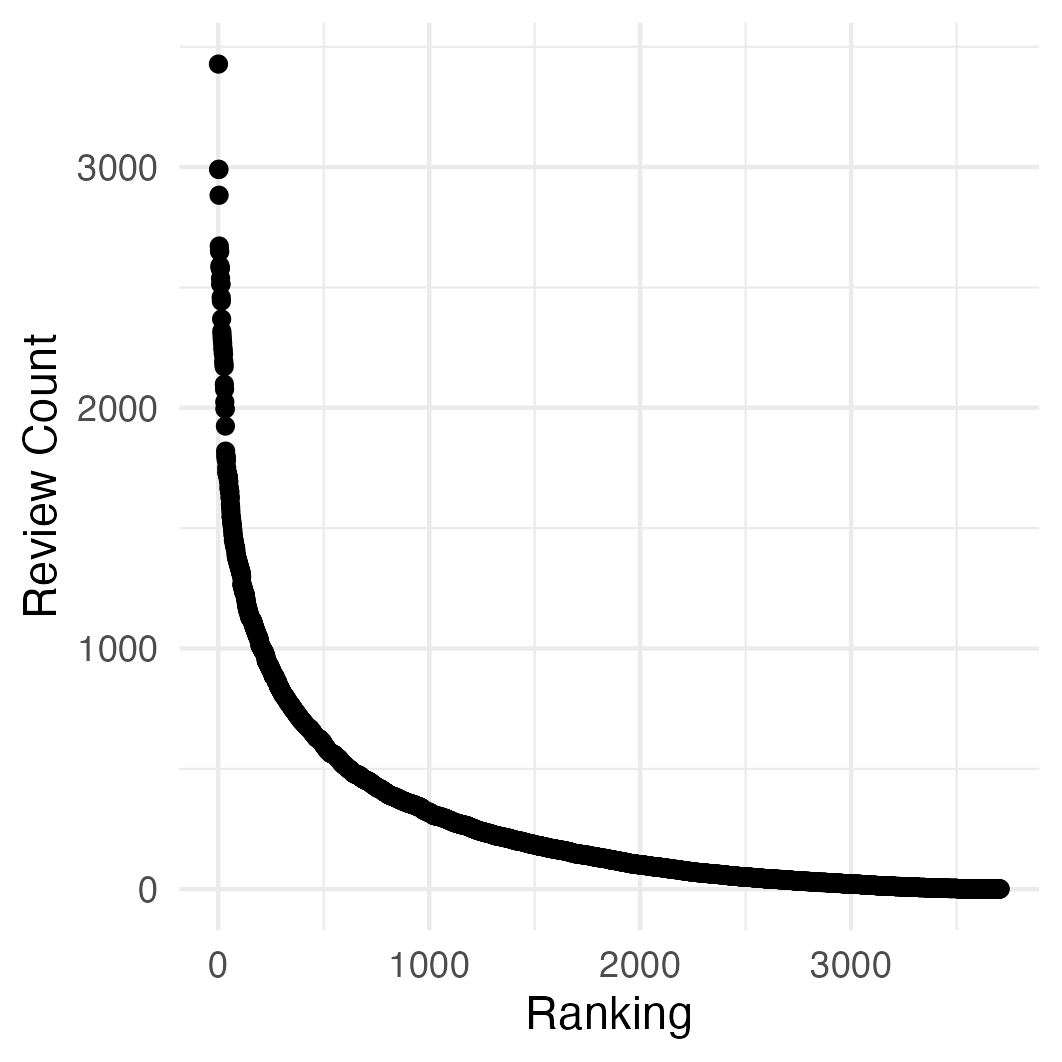
\includegraphics[width=\textwidth]{03_review_profile}
    \caption{Review profile.\label{fig:fig03_review_profile}}
  \end{subfigure}
  \begin{subfigure}{0.45\textwidth}
    \centering
    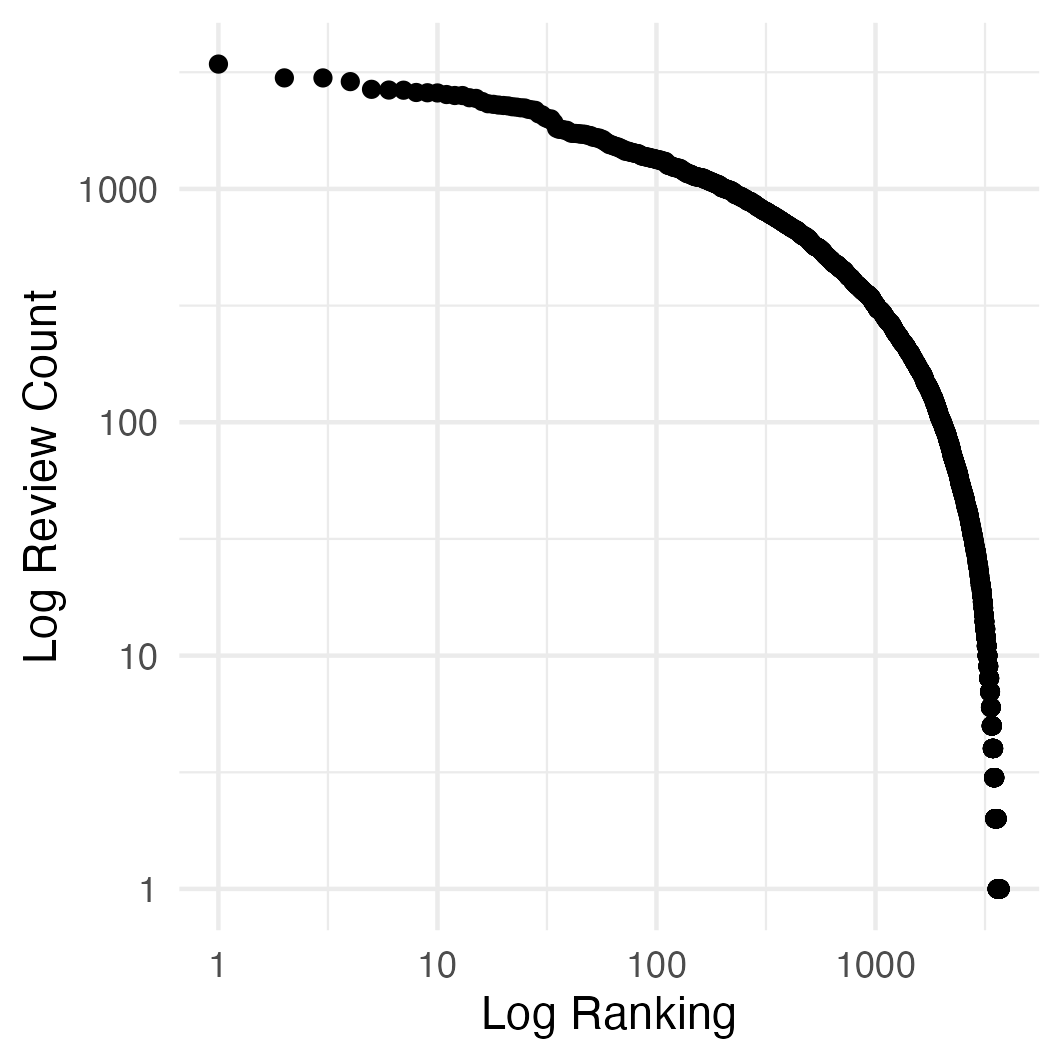
\includegraphics[width=\textwidth]{03_log_review_profile}
    \caption{Log-log plot.\label{fig:fig03_log_review_profile}}
  \end{subfigure}
  \caption{Review profile for the full dataset (a) and log-log
  plot (b).\label{fig:fig03_review_profile_both}}
\end{figure}

\subsection{Trivial Model}
\label{subsec:trivial}

Its recommendation profile can be seen in Figure~\ref{fig:fig1} and, since it is
the sum of many uniform samples, the number of times each movie is recommended
approaches a normal distribution and, therefore, the recommendation profile also
approaches the cumulative distribution function (CDF) of said distribution. The
most recommended movie appeared 25 times in the final list, while the least
recommended movie did not appear at all. Figure~\ref{fig:fig1b} shows the
log-log plot of the recommendation profile.

\begin{figure}
  \centering
  \begin{subfigure}{0.45\textwidth}
    \centering
    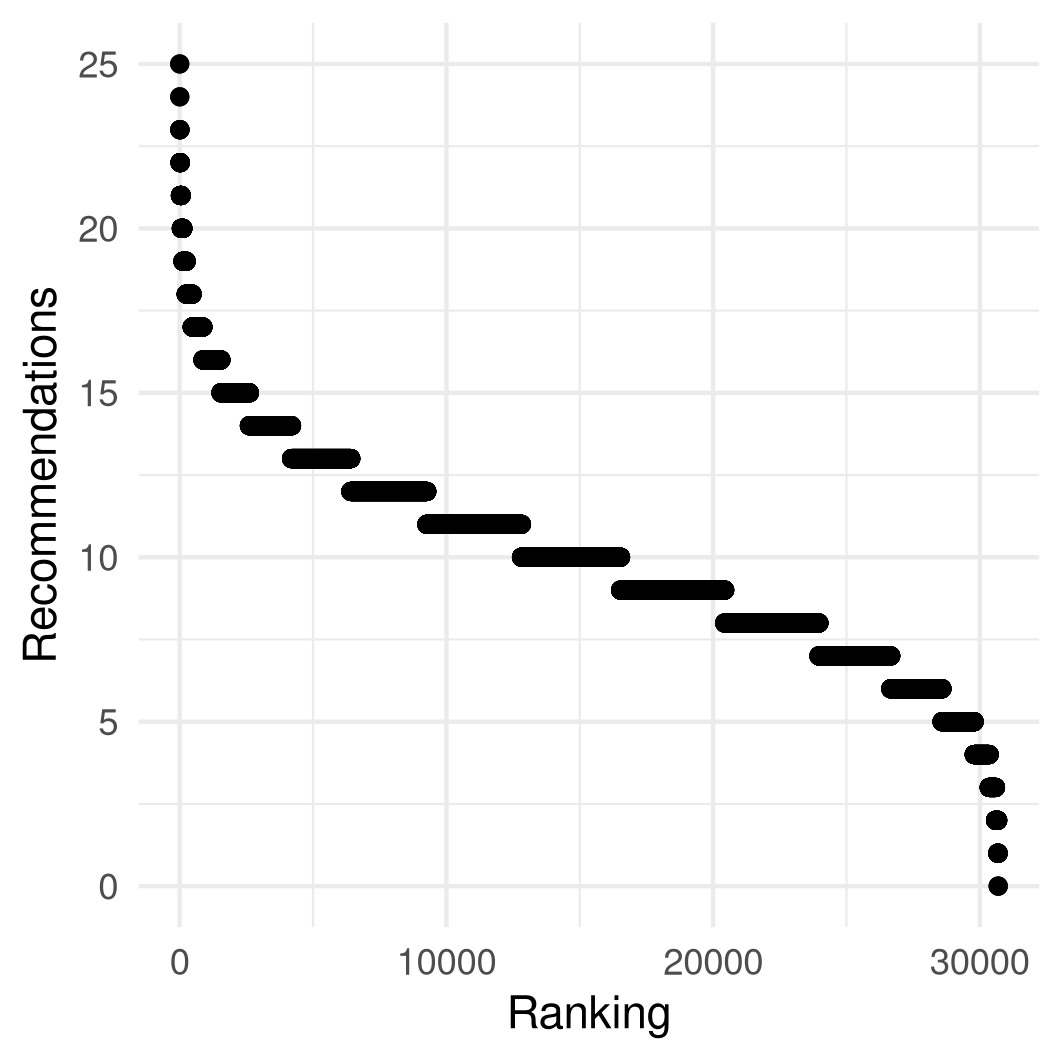
\includegraphics[width=\textwidth]{1a_random}
    \caption{Recommendation profile.\label{fig:fig1a}}
  \end{subfigure}
  \begin{subfigure}{0.45\textwidth}
    \centering
    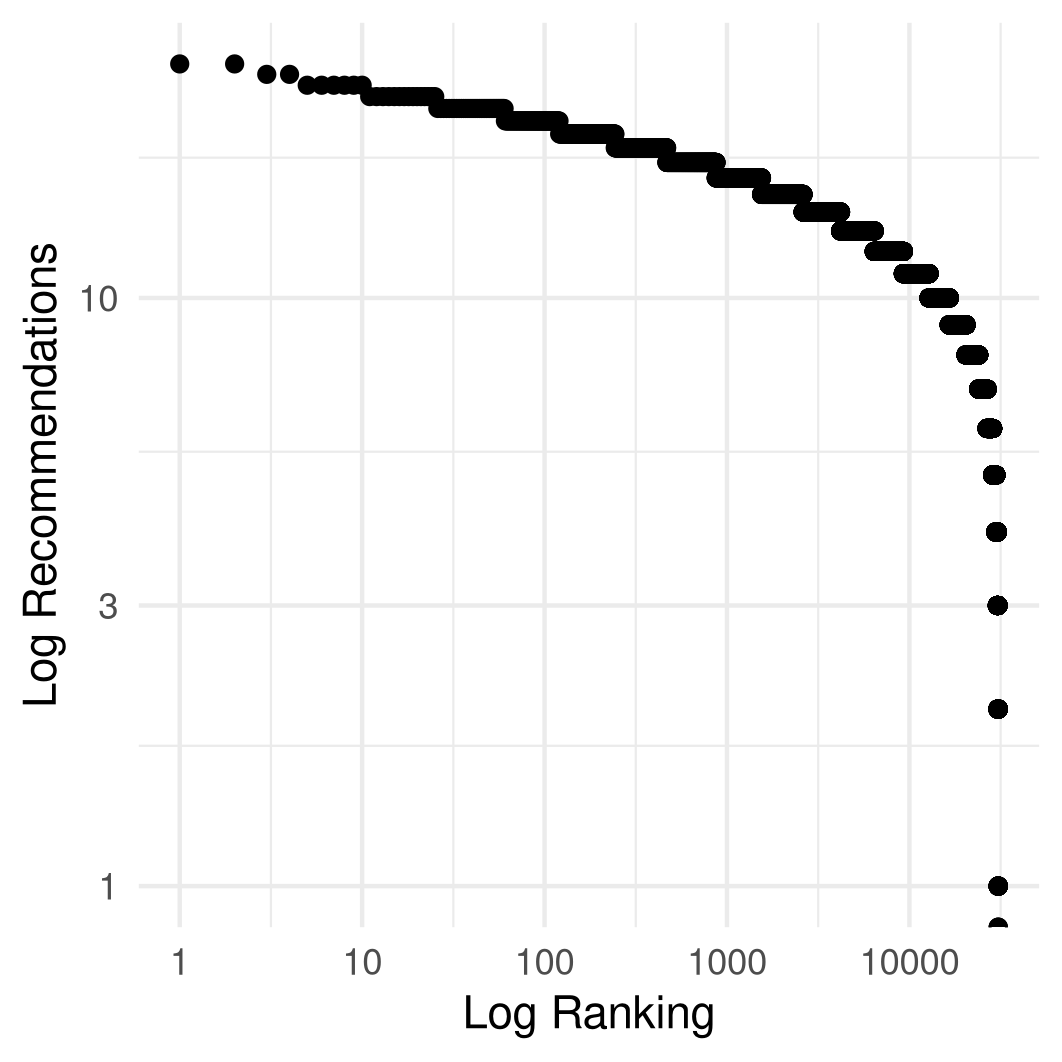
\includegraphics[width=\textwidth]{1b_random_log}
    \caption{Log-log plot.\label{fig:fig1b}}
  \end{subfigure}
  \caption{Recommendation profile for the trivial model (a) and log-log plot
    (b).\label{fig:fig1}}
\end{figure}

\subsection{Vanilla Model}
\label{subsec:vanilla}

The recommendation profile for the vanilla model can be seen in
Figure~\ref{fig:fig2a}. Here, the movie ranked number 1 appeared more than 2000
times in the full list of recommendations, with a power law decay in the number
of appearances from then on, as made evident by the log-log plot on
Figure~\ref{fig:fig2b}. This recommendation profile is a big departure from the
trivial model discussed above.

\begin{figure}
  \centering
  \begin{subfigure}{0.45\textwidth}
    \centering
    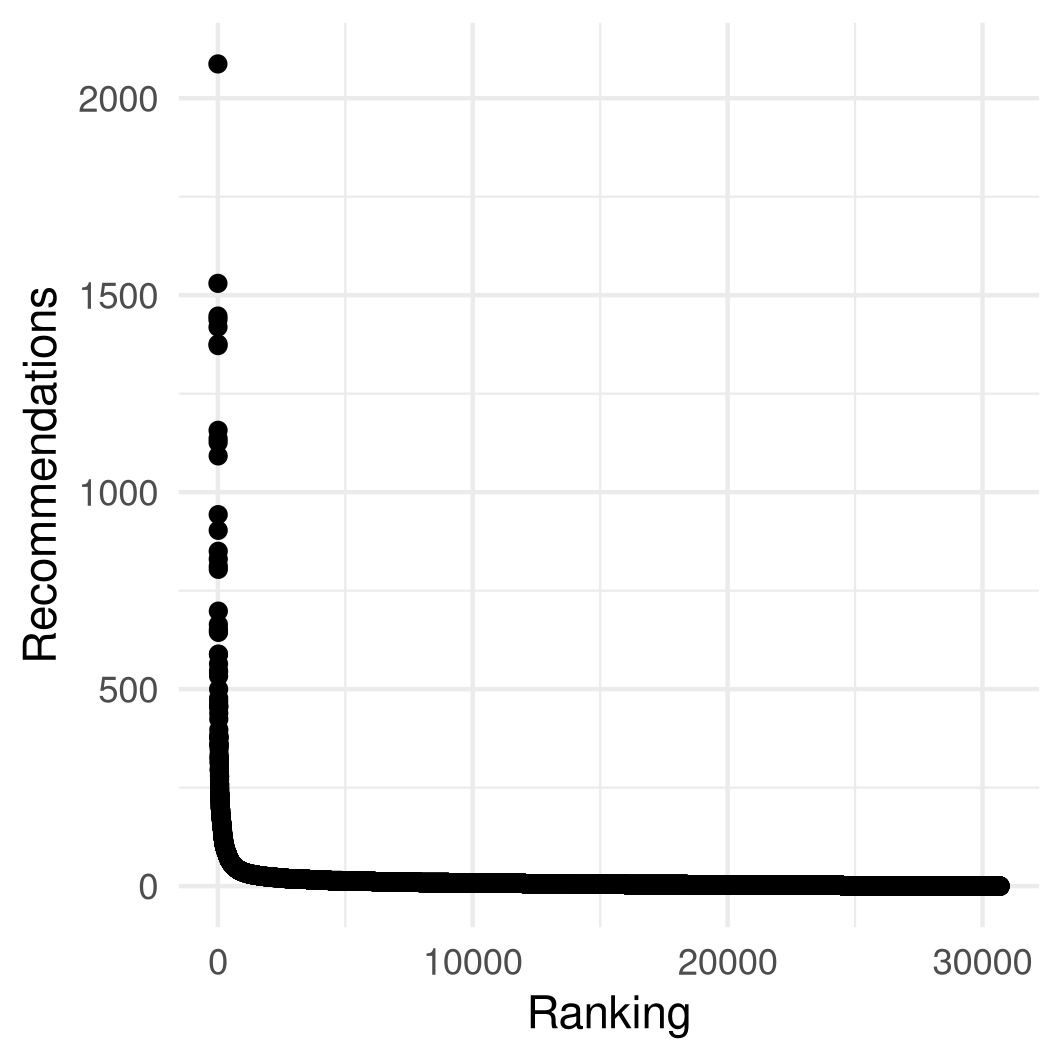
\includegraphics[width=\textwidth]{2a_vanilla}
    \caption{Recommendation profile.\label{fig:fig2a}}
  \end{subfigure}
  \begin{subfigure}{0.45\textwidth}
    \centering
    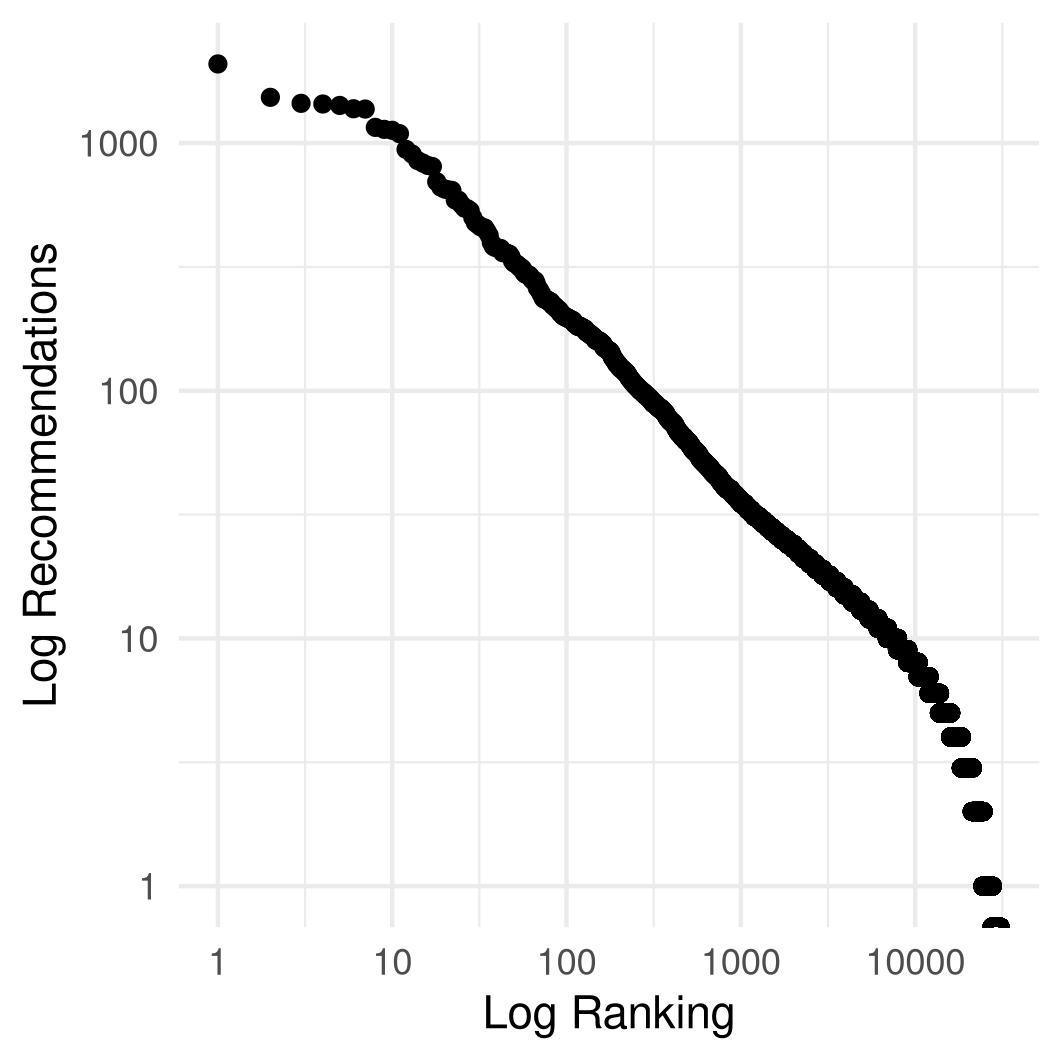
\includegraphics[width=\textwidth]{2b_vanilla_log}
    \caption{Log-log plot.\label{fig:fig2b}}
  \end{subfigure}
  \caption{Recommendation profile for the vanilla model (a) and log-log plot
    (b).\label{fig:fig2}}
\end{figure}

\subsection{Cutoff Models}
\label{subsec:cutoff}

A potential explanation for the difference between trivial and vanilla could
reside in the least used terms in the metadata and that is why we developed the
cutoff model. The results can be seen in Figure~\ref{fig:fig3} and, aside from
variations in the $y$-intercept, all plots are qualitatively very similar to
Figure~\ref{fig:fig2a}, indicating that rare words probably are not to blame for
the power law decay.

\begin{figure}
  \centering
  \begin{subfigure}{0.3\textwidth}
    \centering
    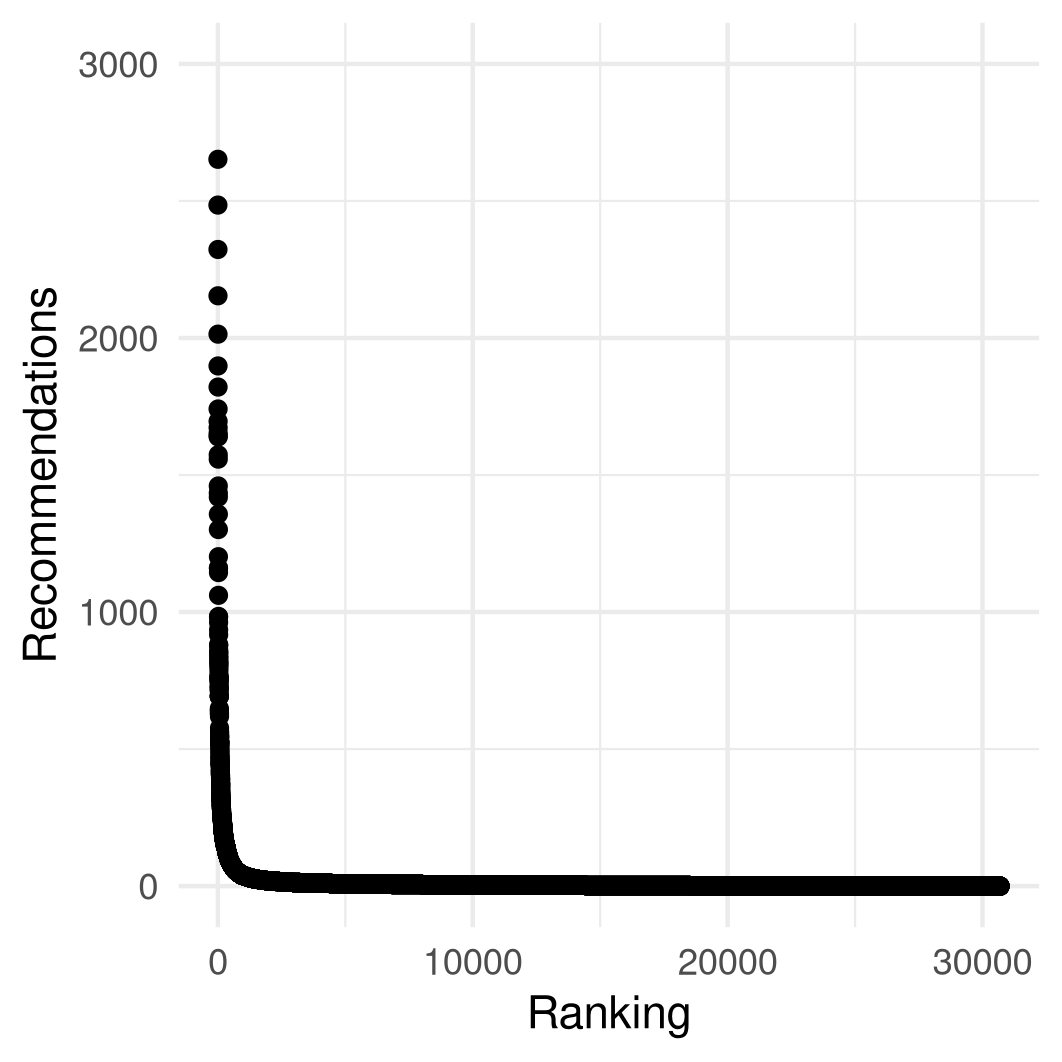
\includegraphics[width=\textwidth]{3a_cutoff_low}
    \caption{Cutoff $k = 2$.\label{fig:fig3a}}
  \end{subfigure}
  \begin{subfigure}{0.3\textwidth}
    \centering
    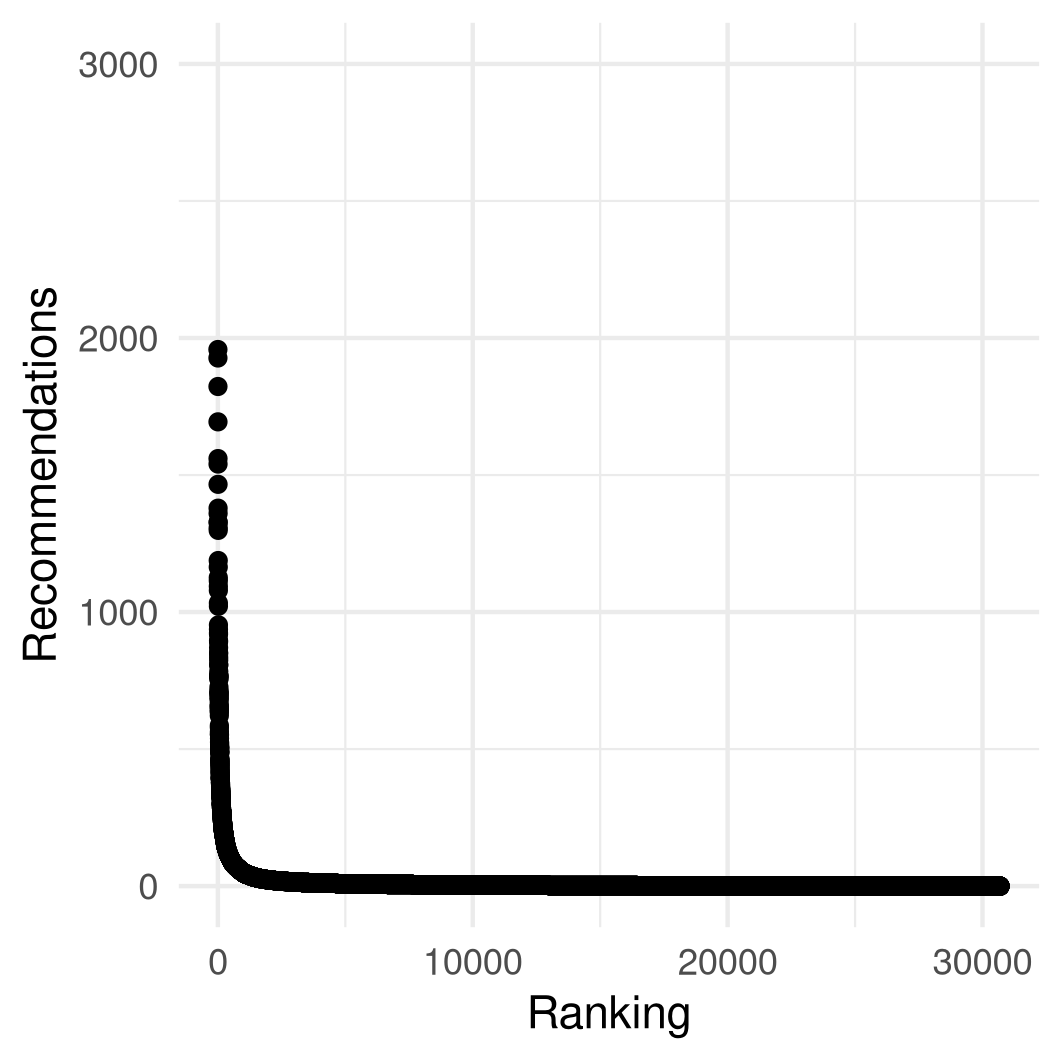
\includegraphics[width=\textwidth]{3b_cutoff_med}
    \caption{Cutoff $k = 5$.\label{fig:fig3b}}
  \end{subfigure}
  \begin{subfigure}{0.3\textwidth}
    \centering
    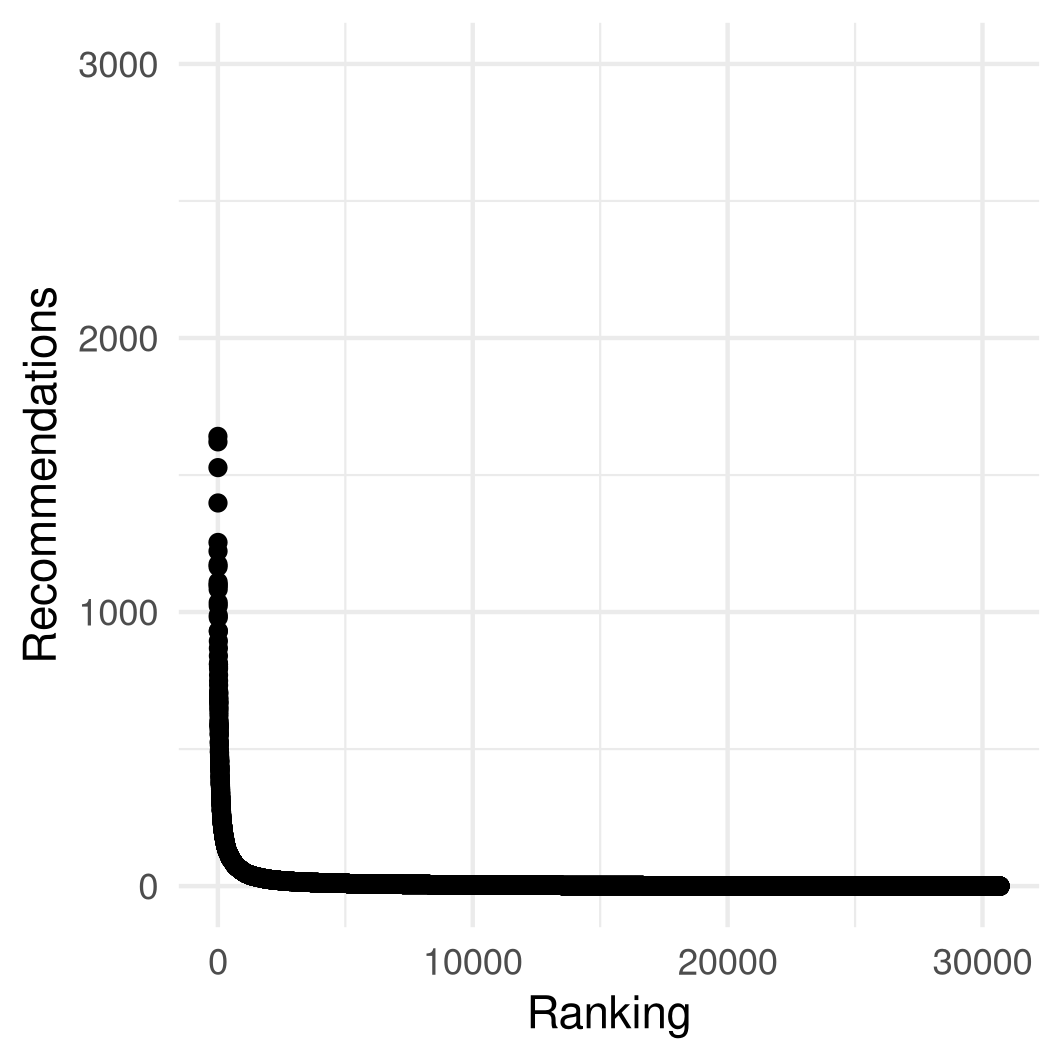
\includegraphics[width=\textwidth]{3c_cutoff_high}
    \caption{Cutoff $k = 8$.\label{fig:fig3c}}
  \end{subfigure}
  \caption{Recommendation profile for cutoff $k = 2$ (a), $5$ (b), and $8$
    (c).\label{fig:fig3}}
\end{figure}

\subsection{Similarity Models}
\label{subsec:similarity}

Since the similarity metric could also be a source of the strange behavior of
the recommendation profile, we conceived the three similarity models described
in the last section. Figure~\ref{fig:fig4} showcases a comparison between cosine
distance, euclidean distance and manhattan distance. It is clear that there are
no meaningful differences between the recommendation profiles generated by each
metric.

\begin{figure}
  \centering
  \begin{subfigure}{0.3\textwidth}
    \centering
    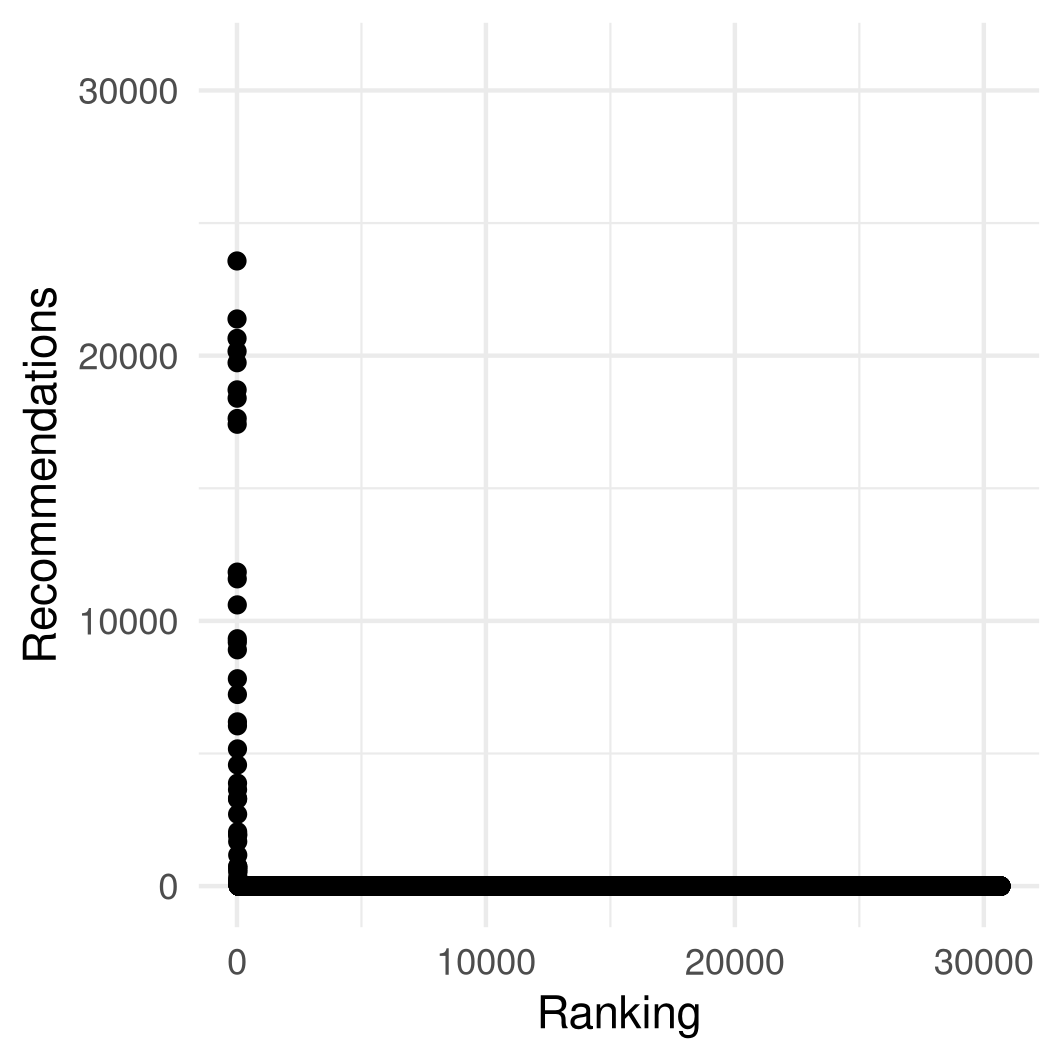
\includegraphics[width=\textwidth]{4a_cosine}
    \caption{Cosine distance (vanilla).\label{fig:fig4a}}
  \end{subfigure}
  \begin{subfigure}{0.3\textwidth}
    \centering
    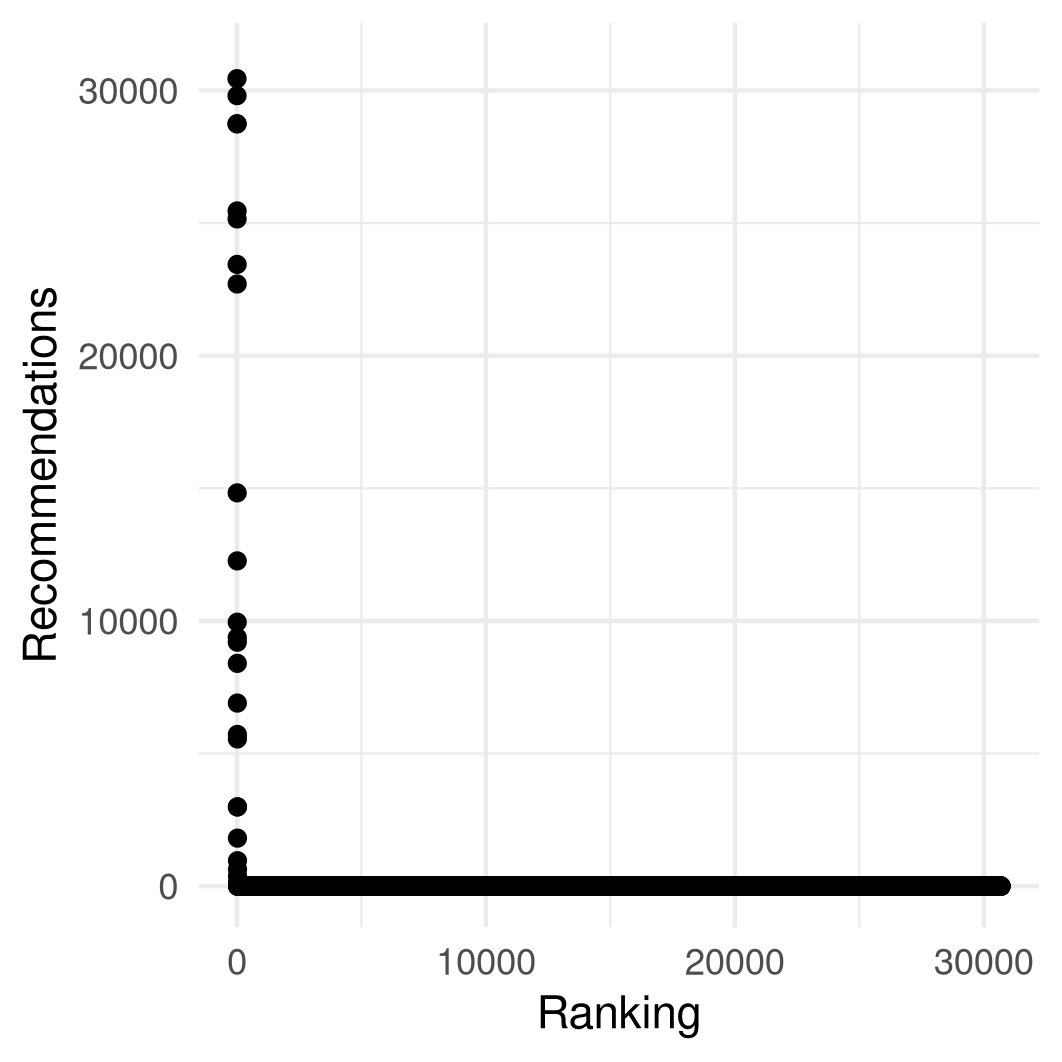
\includegraphics[width=\textwidth]{4b_euclidean}
    \caption{Euclidean distance.\label{fig:fig4b}}
  \end{subfigure}
  \begin{subfigure}{0.3\textwidth}
    \centering
    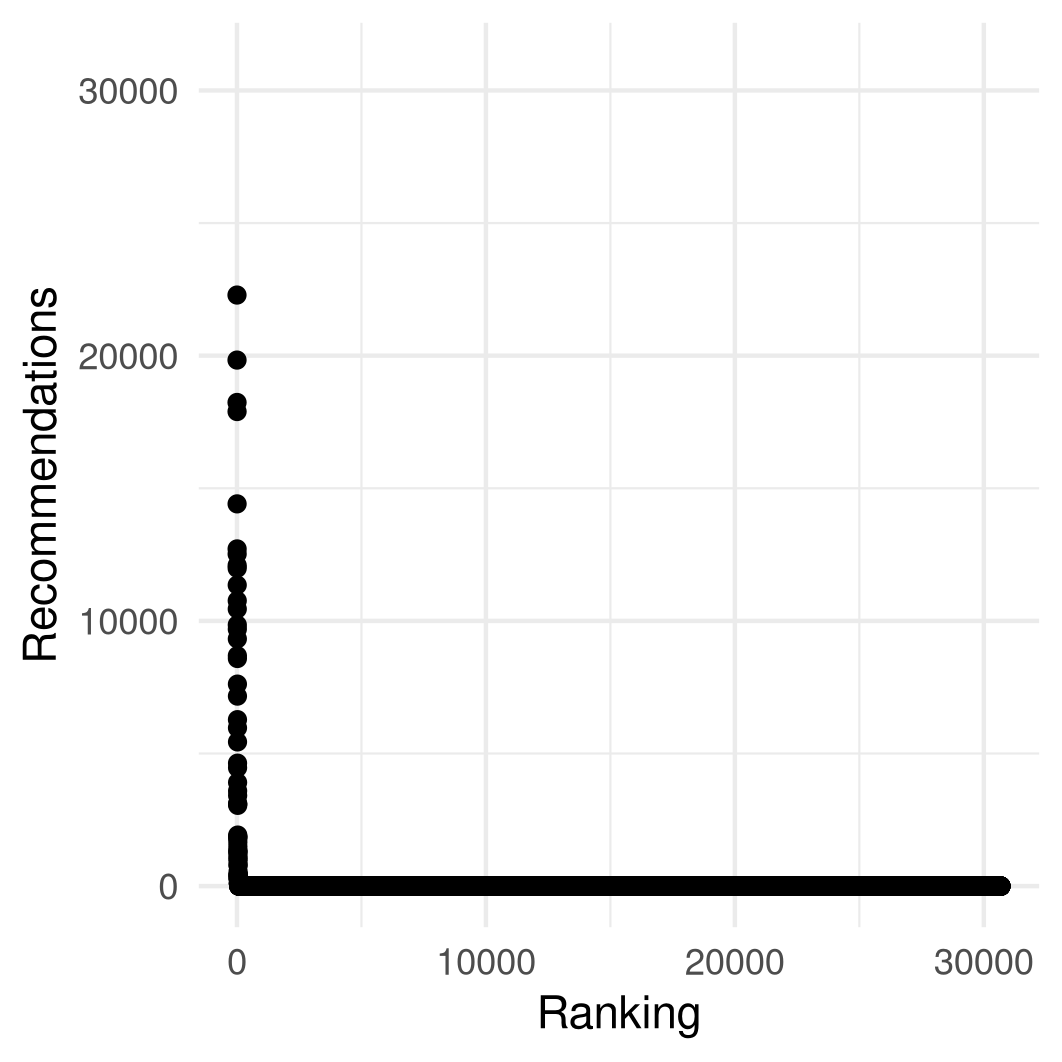
\includegraphics[width=\textwidth]{4c_manhattan}
    \caption{Manhattan distance.\label{fig:fig4c}}
  \end{subfigure}
  \caption{Recommendation profile for cosine (a), euclidean (b), and manhattan
    (c) distances.\label{fig:fig4}}
\end{figure}

\subsection{Vanilla Model with Synthetic Metadata}
\label{subsec:synthetic}

At this point it is safe to say that the type of decay seen in recommendation
frequencies up until now is not spurious and must have a clear cause. To better
investigate whether word frequency had an impact on the recommendation profiles
another hypothesis was taken into consideration: do metadata with less words
cause the recommendation curves to display a steep left-hand side?

Figure~\ref{fig:fig5} displays the recommendation profiles for the vanilla model
applied to datasets with synthetic metadata. Concretely, the figures are
equivalent to creating random metadata for the movies where the probability of
any single word being selected was approximately $1.54 \times 10^{-4}$, $1.54
\times 10^{-3}$, and $1.54 \times 10^{-2}$ respectively. The results do support
the aforementioned hypothesis since denser vectors indeed affected the decay.

\begin{figure}
  \centering
  \begin{subfigure}{0.3\textwidth}
    \centering
    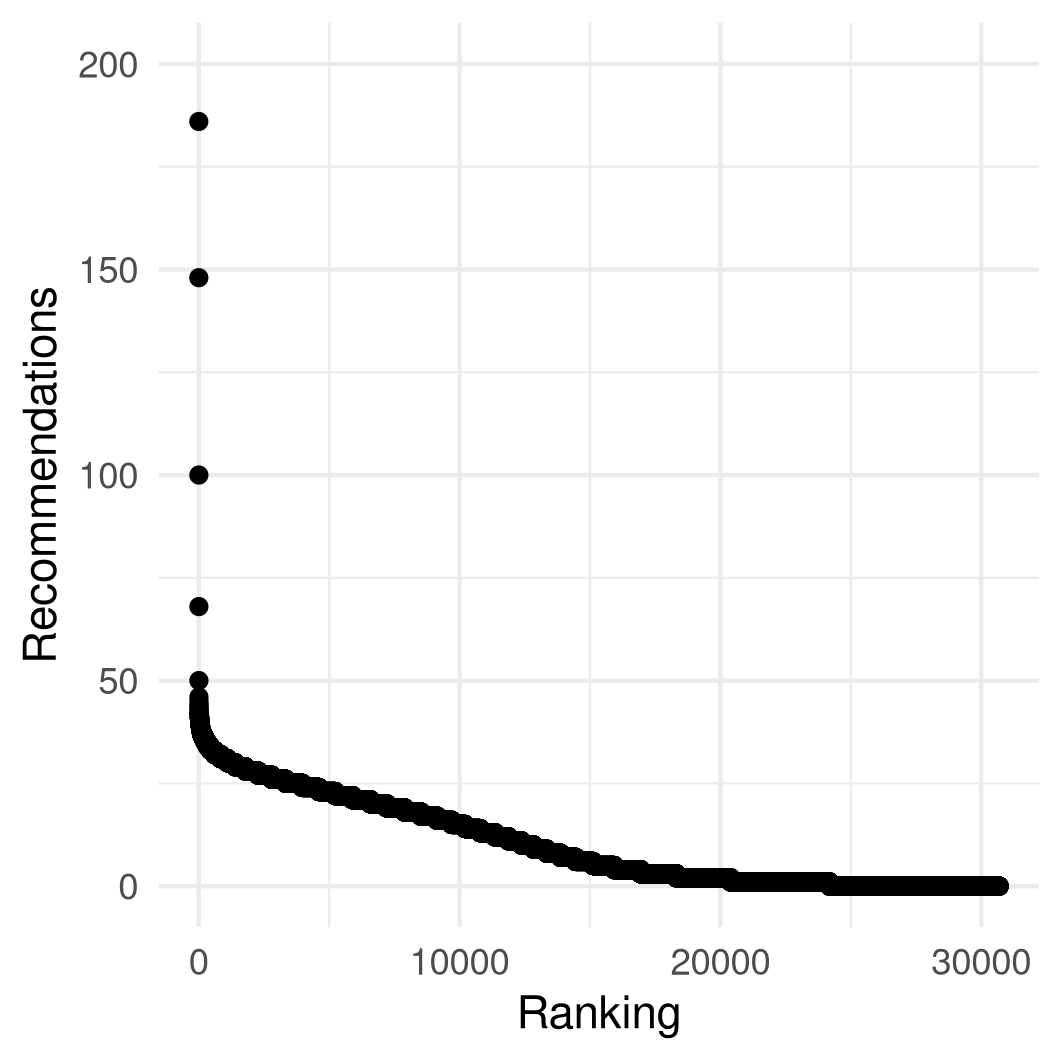
\includegraphics[width=\textwidth]{5a_p}
    \caption{$P(w_{i}) = 1 \times \overline{P(w)}$.\label{fig:fig5a}}
  \end{subfigure}
  \begin{subfigure}{0.3\textwidth}
    \centering
    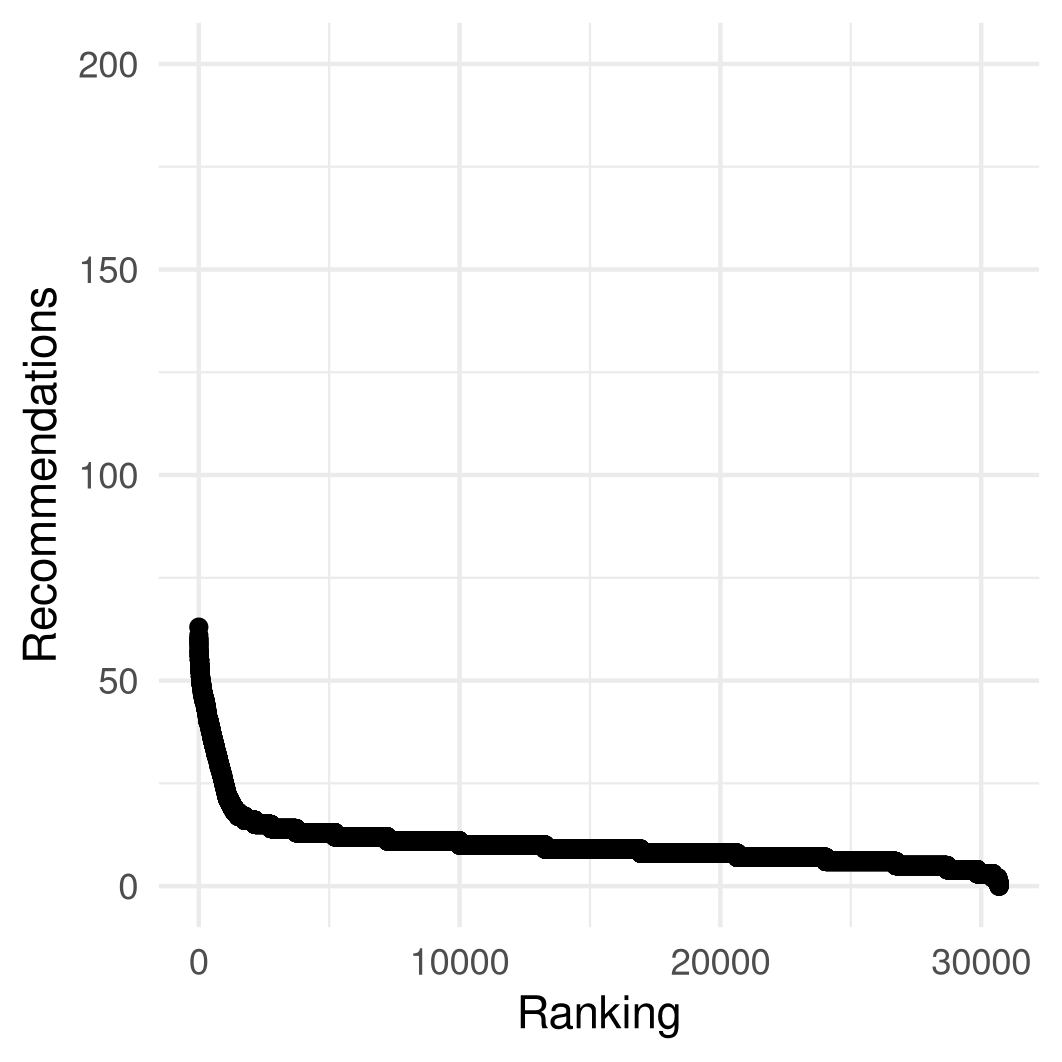
\includegraphics[width=\textwidth]{5b_p10}
    \caption{$P(w_{i}) = 10 \times \overline{P(w)}$.\label{fig:fig5b}}
  \end{subfigure}
  \begin{subfigure}{0.3\textwidth}
    \centering
    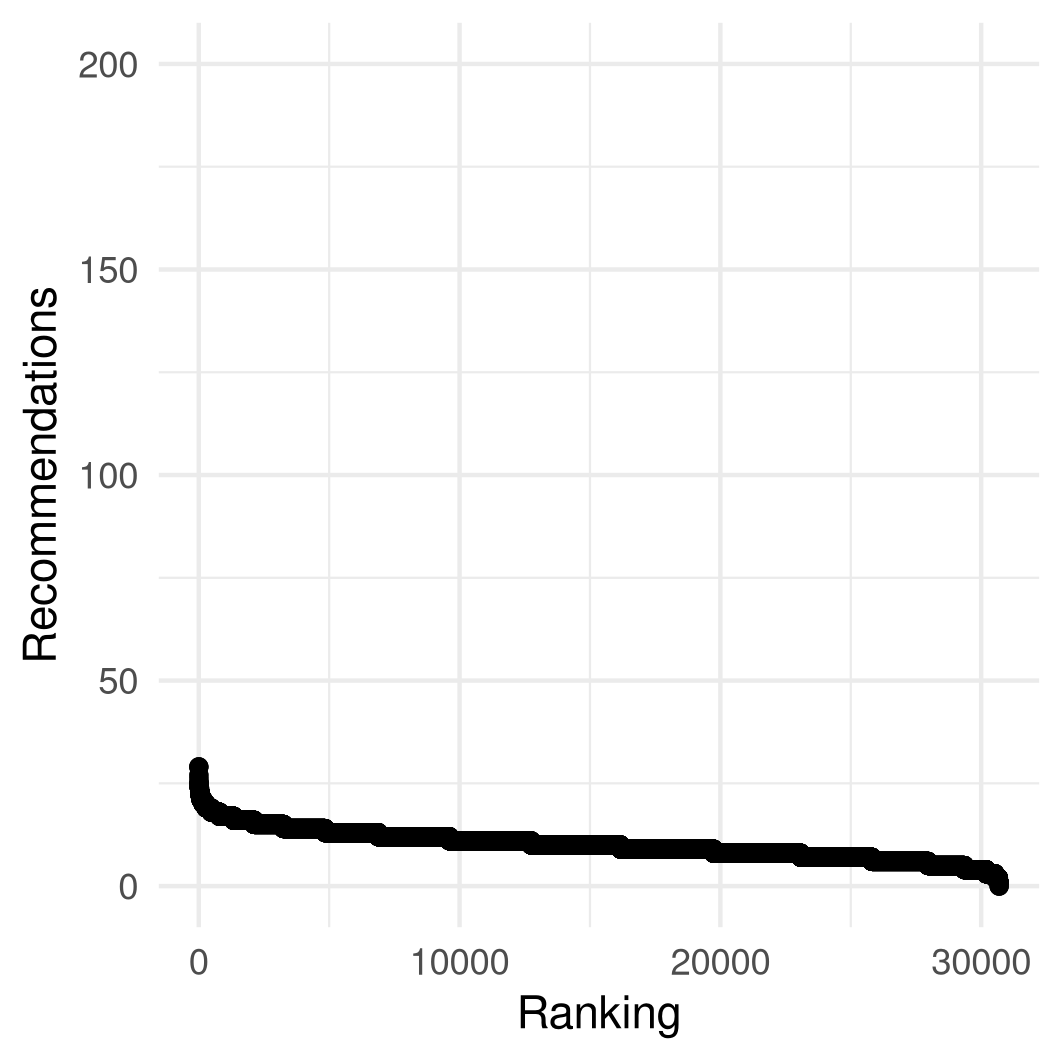
\includegraphics[width=\textwidth]{5c_p100}
    \caption{$P(w_{i}) = 100 \times \overline{P(w)}$.\label{fig:fig5c}}
  \end{subfigure}
  \caption{Recommendation profile of samples with
    $P(w_{i}) = C \times \overline{P(w)}$, $C = 1$ (a), $10$ (b), and $100$
    (c).\label{fig:fig5}}
\end{figure}

\subsection{Sanity Checks}
\label{subsec:sanity03}

After the previous experiments, sanity checks were needed in order to verify
that our previous results weren't spurious. The first check should check whether
an artificial movie created as a combination of the metadata from other movies
favored by the recommendation algorithm would also be favored (i.e. we are able
to create a popular movie from other popular movies), while the second should
check whether shorter vectors would change the decay already observed despite
being as sparse as their longer counterparts (i.e. the intrinsic properties of
the dataset aren't responsible for the power law decay). We repeated these tests
thousands of times and the results presented below are typical of what we found.

Figure~\ref{fig:fig6} showcases the two sanity checks. Figure~\ref{fig:fig6a}
was a model applied to the vanilla dataset with the addition of the movie
highlighted in red. As expected, this movie also showed up in the
top-recommended subset. Figure~\ref{fig:fig6b} comes from a model applied to
randomly generated vector representations in a similar fashion to the ones in
Figure~\ref{fig:fig5}, except each vector could only have 15,000 elements
instead of 55,681 (as with the vanilla model).

\begin{figure}
  \centering
  \begin{subfigure}{0.45\textwidth}
    \centering
    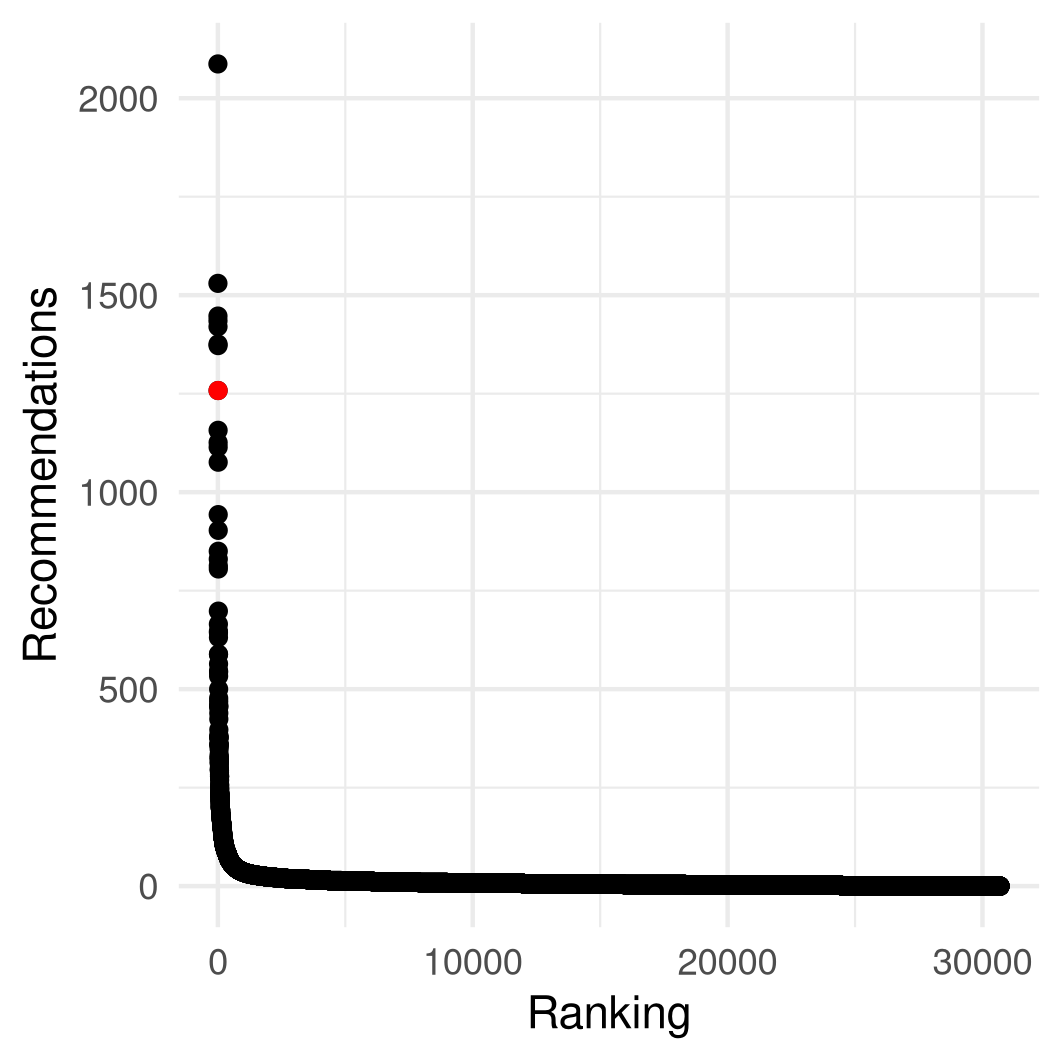
\includegraphics[width=\textwidth]{6a_artificial_movie}
    \caption{Vanilla model with artificial movie in red.\label{fig:fig6a}}
  \end{subfigure}
  \begin{subfigure}{0.45\textwidth}
    \centering
    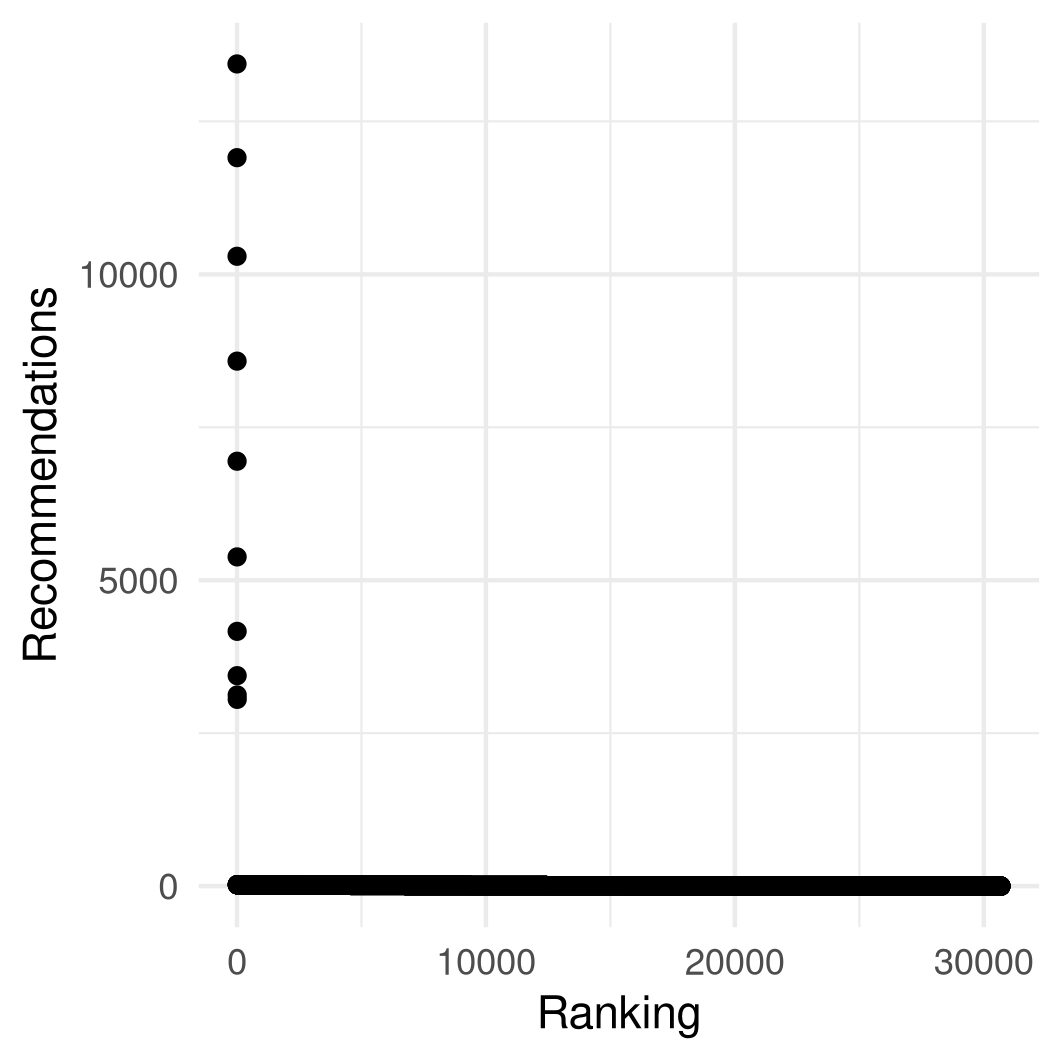
\includegraphics[width=\textwidth]{6b_long}
    \caption{Model with short vector representations.\label{fig:fig6b}}
  \end{subfigure}
  \caption{Recommendation profile for artificial movie (a) and short vector
    representations (b).\label{fig:fig6}}
\end{figure}

The last two models were considered the confirmations of the hypothesis that (at
least for this kind of recommendation systems) a subset of items was always much
more recommended than the rest as long as the data was sparse.
Figure~\ref{fig:fig7a} represents the same recommendation algorithm applied to
another dataset, the Book-Crossing dataset. Figure~\ref{fig:fig7b} contains the
results of the model applied to another set of random vector representations,
this time with the probability of each element being non-zero respecting the
marginal distributions of the vanilla dataset. Again, the power law decay
pattern persisted, only slightly less pronounced in the Book-Crossing case.

\begin{figure}
  \centering
  \begin{subfigure}{0.45\textwidth}
    \centering
    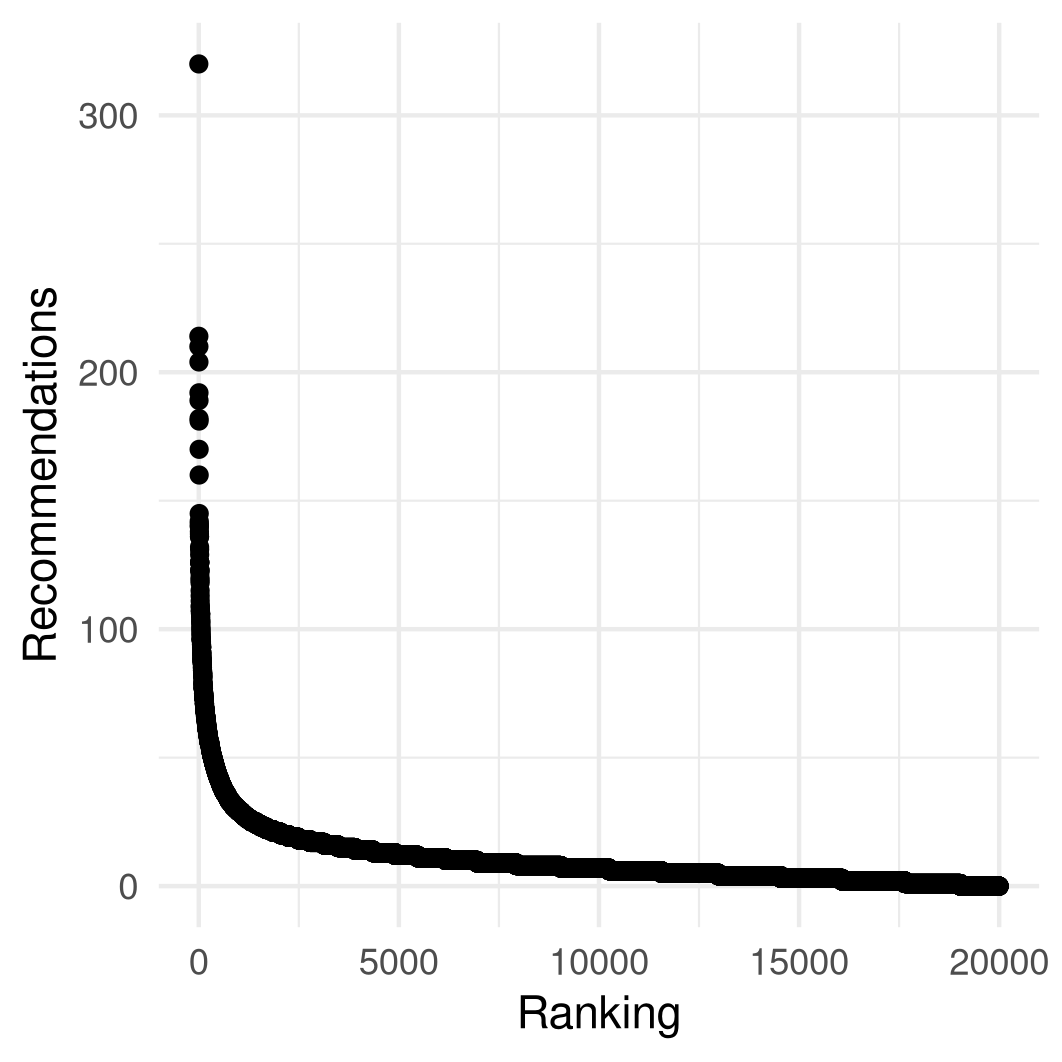
\includegraphics[width=\textwidth]{7a_books}
    \caption{Recommendation profile for book dataset.\label{fig:fig7a}}
  \end{subfigure}
  \begin{subfigure}{0.45\textwidth}
    \centering
    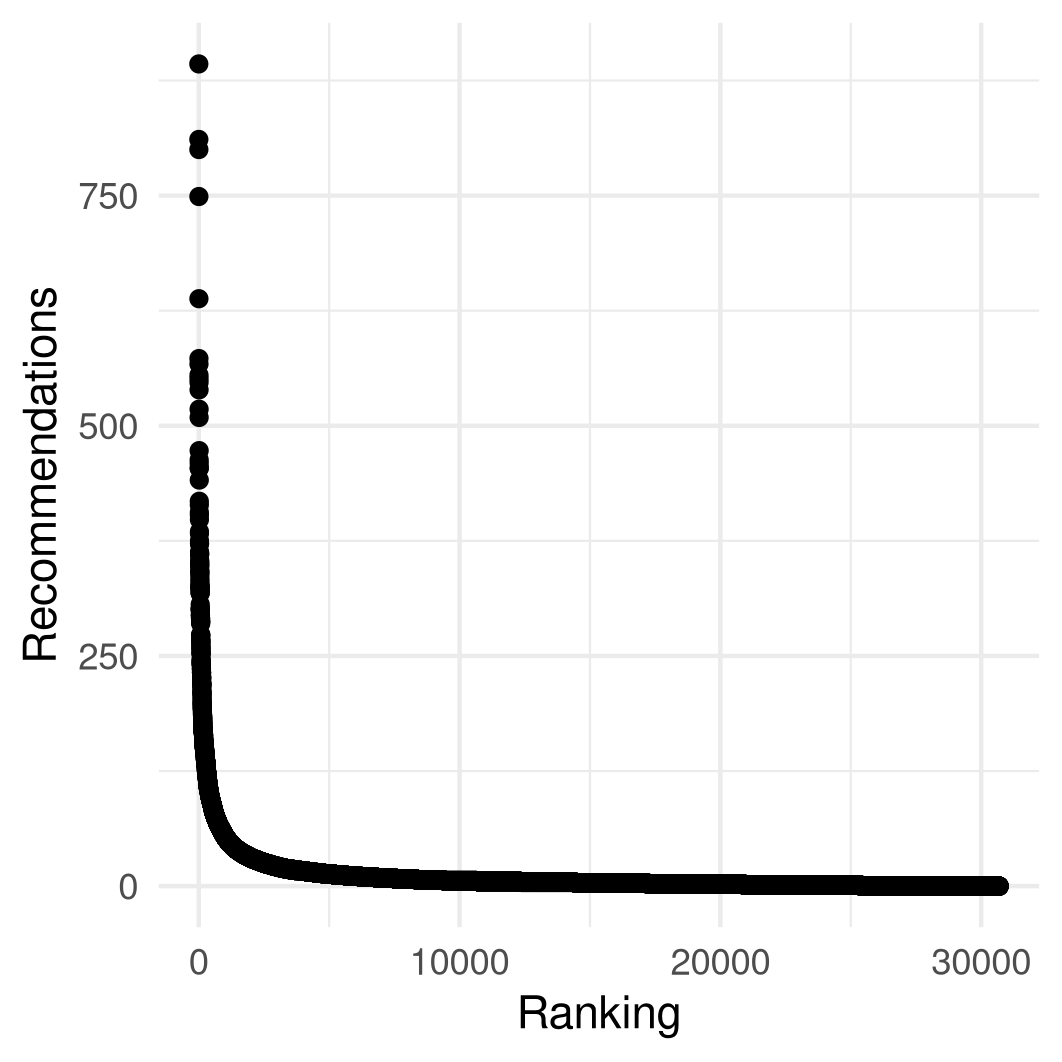
\includegraphics[width=\textwidth]{7b_mimic}
    \caption{Random simularion of vanilla.\label{fig:fig7b}}
  \end{subfigure}
  \caption{Recommendation profile for book dataset (a) and random simulation of
    vanilla (b).\label{fig:fig7}}
\end{figure}

The analysis up until now has been static, that is, the recommendation model
does not learn from the users' responses to its suggestions. There is no
interaction with users and no opportunity to evolve over time. The next chapter
addresses this point by using Google's newly released TensorFlow Recommenders
library \citep{noauthor_tensorflow_nodate} to gather data about what happens to
a system's recommendations as users follow its suggestions. Employing a deep
learning model that is able to improve over time is a significant departure from
the content-based models presented here and, if a similar recommendation profile
can also be detected for multi-criteria recommender systems on dynamic
scenarios, then the hypothesis ventilated in the section above would become even
more plausible.

\par

%!TeX root=../tese.tex
%("dica" para o editor de texto: este arquivo é parte de um documento maior)
% para saber mais: https://tex.stackexchange.com/q/78101/183146

\chapter{Dynamic Analysis}
\label{cap:dynamic}

Following the static analysis, it became clear that a dynamic analysis would be
of the utmost importance. Understanding how the recommendation model responds to
users reinforcing its internal biases, like the ones already detected, could
potentially lead to a better understanding of how these systems favor certain
kinds of content.

In order for this analysis to be more true to reality, we implemented a simple
recommendation algorithm using TensorFlow Recommenders \citep{}, a library for
machine learning developed by Google for use with its TensorFlow \citep{}
framework. This means that, even though our model is deliberately bare-bones, it
conforms to industry-standard technology and practices.

The choice to use a simple recommendation algorithm instead of a more complex
one was twofold: first, we didn't want to use a model that could introduce many
confounding parameters to the analysis (e.g. hyperparameters, hardware
requirements, etc.), and second, we wanted to study a baseline that could, in
the future, be used as a comparison point for more complex algorithms.

The goal of this analysis is to gather data on how the recommendation system
behaves over time. As will be explained in the next sections, is to understand
what happens to the recommendation profile of the algorithm as it interacts with
itself via users that follow the generated suggestions.

The expectation is that the recommendation profile will grow ever more steep,
which is a reasonable guess; if the users reinforce the beliefs of the
algorithm, then is stands to reason that it will recommend popular movies with
more and more frequently, to more and more users. How much more frequently,
however, is the true question.

For the sake of clarity, let's imagine two users with very distinct preferences:
Alice, who enjoys adventure movies, and Bob, who enjoys horror movies. In
principle, the algorithm should have very different recommendations for both of
them and, were they to follow them, their custom suggestions should grow
increasingly different. At the end of this experiment, users like Alice would
all be recommended the same movies, and users like Bob would have their own set
of very popular films; we should expect, therefore, a multimodal distribution of
the recommendation frequencies, with "typical" adventure movies and "typical"
horror movies being much more popular than comedy, for example.

However, if the final recommendation profile looked like what was showcased in
the previous chapter, i.e. a very small subset of movies being recommended to
most users, then we could infer that the system devolved into a degenerate
feedback loop, ignoring personal preferences and distinctions between films.

\section{Datasets}
\label{sec:datasets04}

For the dynamic experiments, we kept using the Movielens dataset \citep{}. This
time, however, we used the full ``1M'' dataset instead of sampling movies from
the larger ``25M'' version. Given that we wanted our dynamic analysis to be
conducted in a realistic scenario, we decided that it would be better not to
change the data. This whole experiment will, therefore, use a version of the
dataset commonly used for machine learning benchmarks with no alteration
whatsoever.

The 1M dataset contains 1,000,209 ratings of almost 4000 movies made by over
6000 anonymous MovieLens users who joined the platform in 2000. In this
particular version, each user has made at least 20 ratings. There are 4 columns
available:

\begin{itemize}
  \item \verb|UserID|: Unique user identifier, ranging from 1 to 6040.
  \item \verb|MovieID|: Unique movie identifier, ranging from 1 to 3952.
  \item \verb|Rating|: Movie rating according to user, from 0 to 5 stars.
  \item \verb|Timestamp|: When the user made the rating, in seconds since the
  epoch.
\end{itemize}

A second, auxiliary, dataset was also used to enrich the main one. ``Movies''
contains extra information about the movies in 1M, which allowed us to add more
variables to the recommendation system. This new dataset has 3 columns:

\begin{itemize}
  \item \verb|MovieID|: Unique user identifier, ranging from 1 to 6040.
  \item \verb|Title|: Title of the movie, as provided by IMDB.
  \item \verb|Genres|: Pipe-separated string with all applicable genres.
\end{itemize}

The other accompanying dataset, ``Users'', has not been used for the purposes of
this analysis. The reasoning behind this decision will be explained in greater
detail in the next section.

\section{Experiments}
\label{sec:experiments04}

The dynamic experiment starts in a manner much similar to the static experiment.
The full MovieLens dataset is fed as training data to a recommendation system in
order to get it ready for giving suggestions to users. As explained in the
opening section of this chapter, we chose a simple algorithm in order to reduce
the number of possible interferences architecture could have on our analysis.

The chosen recommendation algorithm was a basic ranking model described in
\citet{} using TensorFlow Recommenders \citep{}. It is composed of multiple
stacked dense layers and uses mean squared error as its loss function. The main
class in the model is reproduced below, and the full algorithm is listed in
Appendix~\ref{}.

%% Deixar o código em pseudo-código para ficar mais claro

\begin{verbatim}
class MovielensModel(tfrs.models.Model):

  def __init__(self):
    super().__init__()
    self.ranking_model: tf.keras.Model = RankingModel()
    self.task: tf.keras.layers.Layer = tfrs.tasks.Ranking(
      loss = tf.keras.losses.MeanSquaredError(),
      metrics=[tf.keras.metrics.RootMeanSquaredError()]
    )

  def call(self, features: Dict[str, tf.Tensor]) -> tf.Tensor:
    return self.ranking_model(
        (features["user_id"], features["movie_title"]))

  def compute_loss(self, features: Dict[Text, tf.Tensor],
                    training=False) -> tf.Tensor:
    labels = features.pop("user_rating")

    rating_predictions = self(features)

    # The task computes the loss and the metrics.
    return self.task(labels=labels, predictions=rating_predictions)
\end{verbatim}

In the first step of the experiment, we trained the recommendation model using
Movielens' 1M ratings dataset, which we will refer to as \verb|ratings0| from
now on. All available data was used and, in the end, we achieved a root mean
squared error (RMSE) of 0.92; this result is similar to TFRS' deep \& cross
network \citep{} results when trained on the same data. Once \verb|model0| was
ready for making recommendations, we applied it to every possible user-movie
pairing, generating a complete matrix of predicted ratings called
\verb|predictions0|.

In an environment like YouTube's recommendations sidebar, the user is presented
with a few items that the algorithm thinks they would like, and then they can
either ignore the sidebar or select one of the options to watch. Since our goal
was to explore what would happen when the recommendation system entered a
feedback loop, we picked one movie at random from each user's 10 best-ranked
entries.

This set of well-ranked movies was our way of simulating thousands of users
simultaneously approving of the algorithms recommendations and selecting one
option from their sidebars. The last step involved removing the oldest rating of
each each user from \verb|ratings0| and appending these these selections to the
dataset in order to create \verb|ratings1|. The full data flow is illustrated
in Figure~\ref{fig:fig04_dynamic_diagram}

\begin{figure}
  \centering
  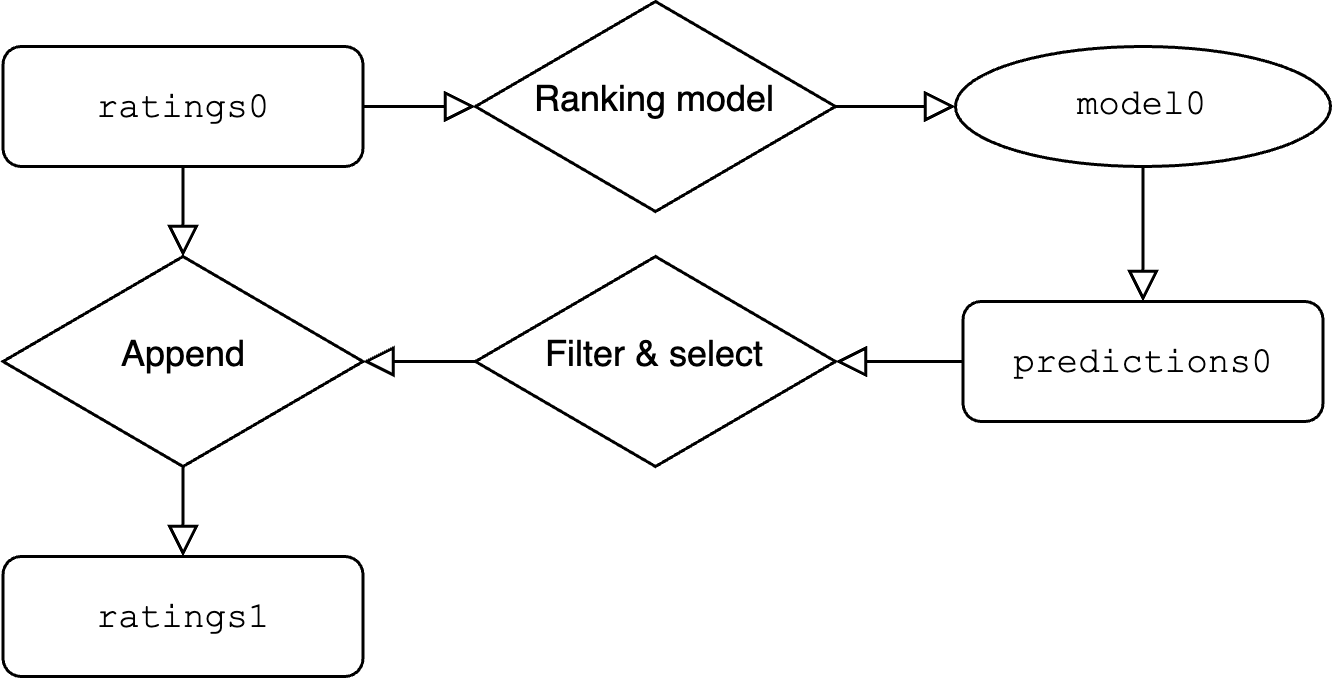
\includegraphics[width=\textwidth]{04_dynamic_diagram}
  \caption{Data flow diagram.\label{fig:fig04_dynamic_diagram}}
\end{figure}

% Explicar o que são os formatos no caption da figura.

A feedback loop, however, can't be created from a single iteration. For this
reason, the process just described was classified as the ``zeroth'' iteration in
the process (as it involved \verb|ratings0|). The ``first'' iteration began with
\verb|ratings1|, trained \verb|model1|, generated \verb|predictions1|, and ended
with \verb|ratings2|. We repeated this process until we got to \verb|ratings4|,
totaling 5 ratings datasets (one original and 4 derived through ranking models).

A simplified version of the R code that created \verb|ratingsN+1| from
\verb|ratingsN| can be found below. The omitted functions served mostly
auxiliary purposes which made the datasets conform to TensorFlow's format
expectations. The full code is listed in Appendix~\ref{}.

\begin{verbatim}
predictions |>
  group_by(user_id) |>
  slice_max(prediction, n = 10) |>
  slice_sample(n = 1) |>
  ungroup() |>
  bind_rows(old_ratings) |>
  group_by(user_id) |>
  slice_max(timestamp, n = -1, with_ties = FALSE) |>
  ungroup()
\end{verbatim}

With these new datasets we were able to analyze the differences between distinct
generations of models and understand exactly how the positive feedback loop
influenced the last iteration.

A series of analysis were conducted using these datasets as sources. We found
that, with each iteration, the recommendation profile got steeper and steeper,
that is, a few popular items got more recommended while the rest fell into
disfavor; this was predictably more noticeable in movies with higher average
ratings. In fact, a small set of around 20 movies were the only ones that
consistently rose in popularity with new iterations.

Figure~\ref{fig:fig04_profile_grouped} has five subplots which represent each
iteration of the recommendation system. For \verb|ratings0|, it's possible to
see that a number of well-rated movies were more popular, i.e., were rated by
more people. Once we generate the first batch of recommendations, we add up the
number of users each movie was recommended to; this is seen in the second plot,
\verb|ratings1|. We can clearly see that a small subset of movies strayed from
the pack and to more people that had watched them previously.

This process repeats itself until, in \verb|ratings4|, the most popular movie is
recommended more than 2000 times, while the most popular movie in
\verb|ratings0| was watched a little over 500 times.

As explained before, we expected that movies which where already popular would
be recommended more times, but these plots indicate a powerful feedback loop.
Examining the data, we saw that the algorithm was consistently recommending
movies which the users had already watched and this process only became more
accentuated with each subsequent iteration.

\begin{figure}
  \centering
  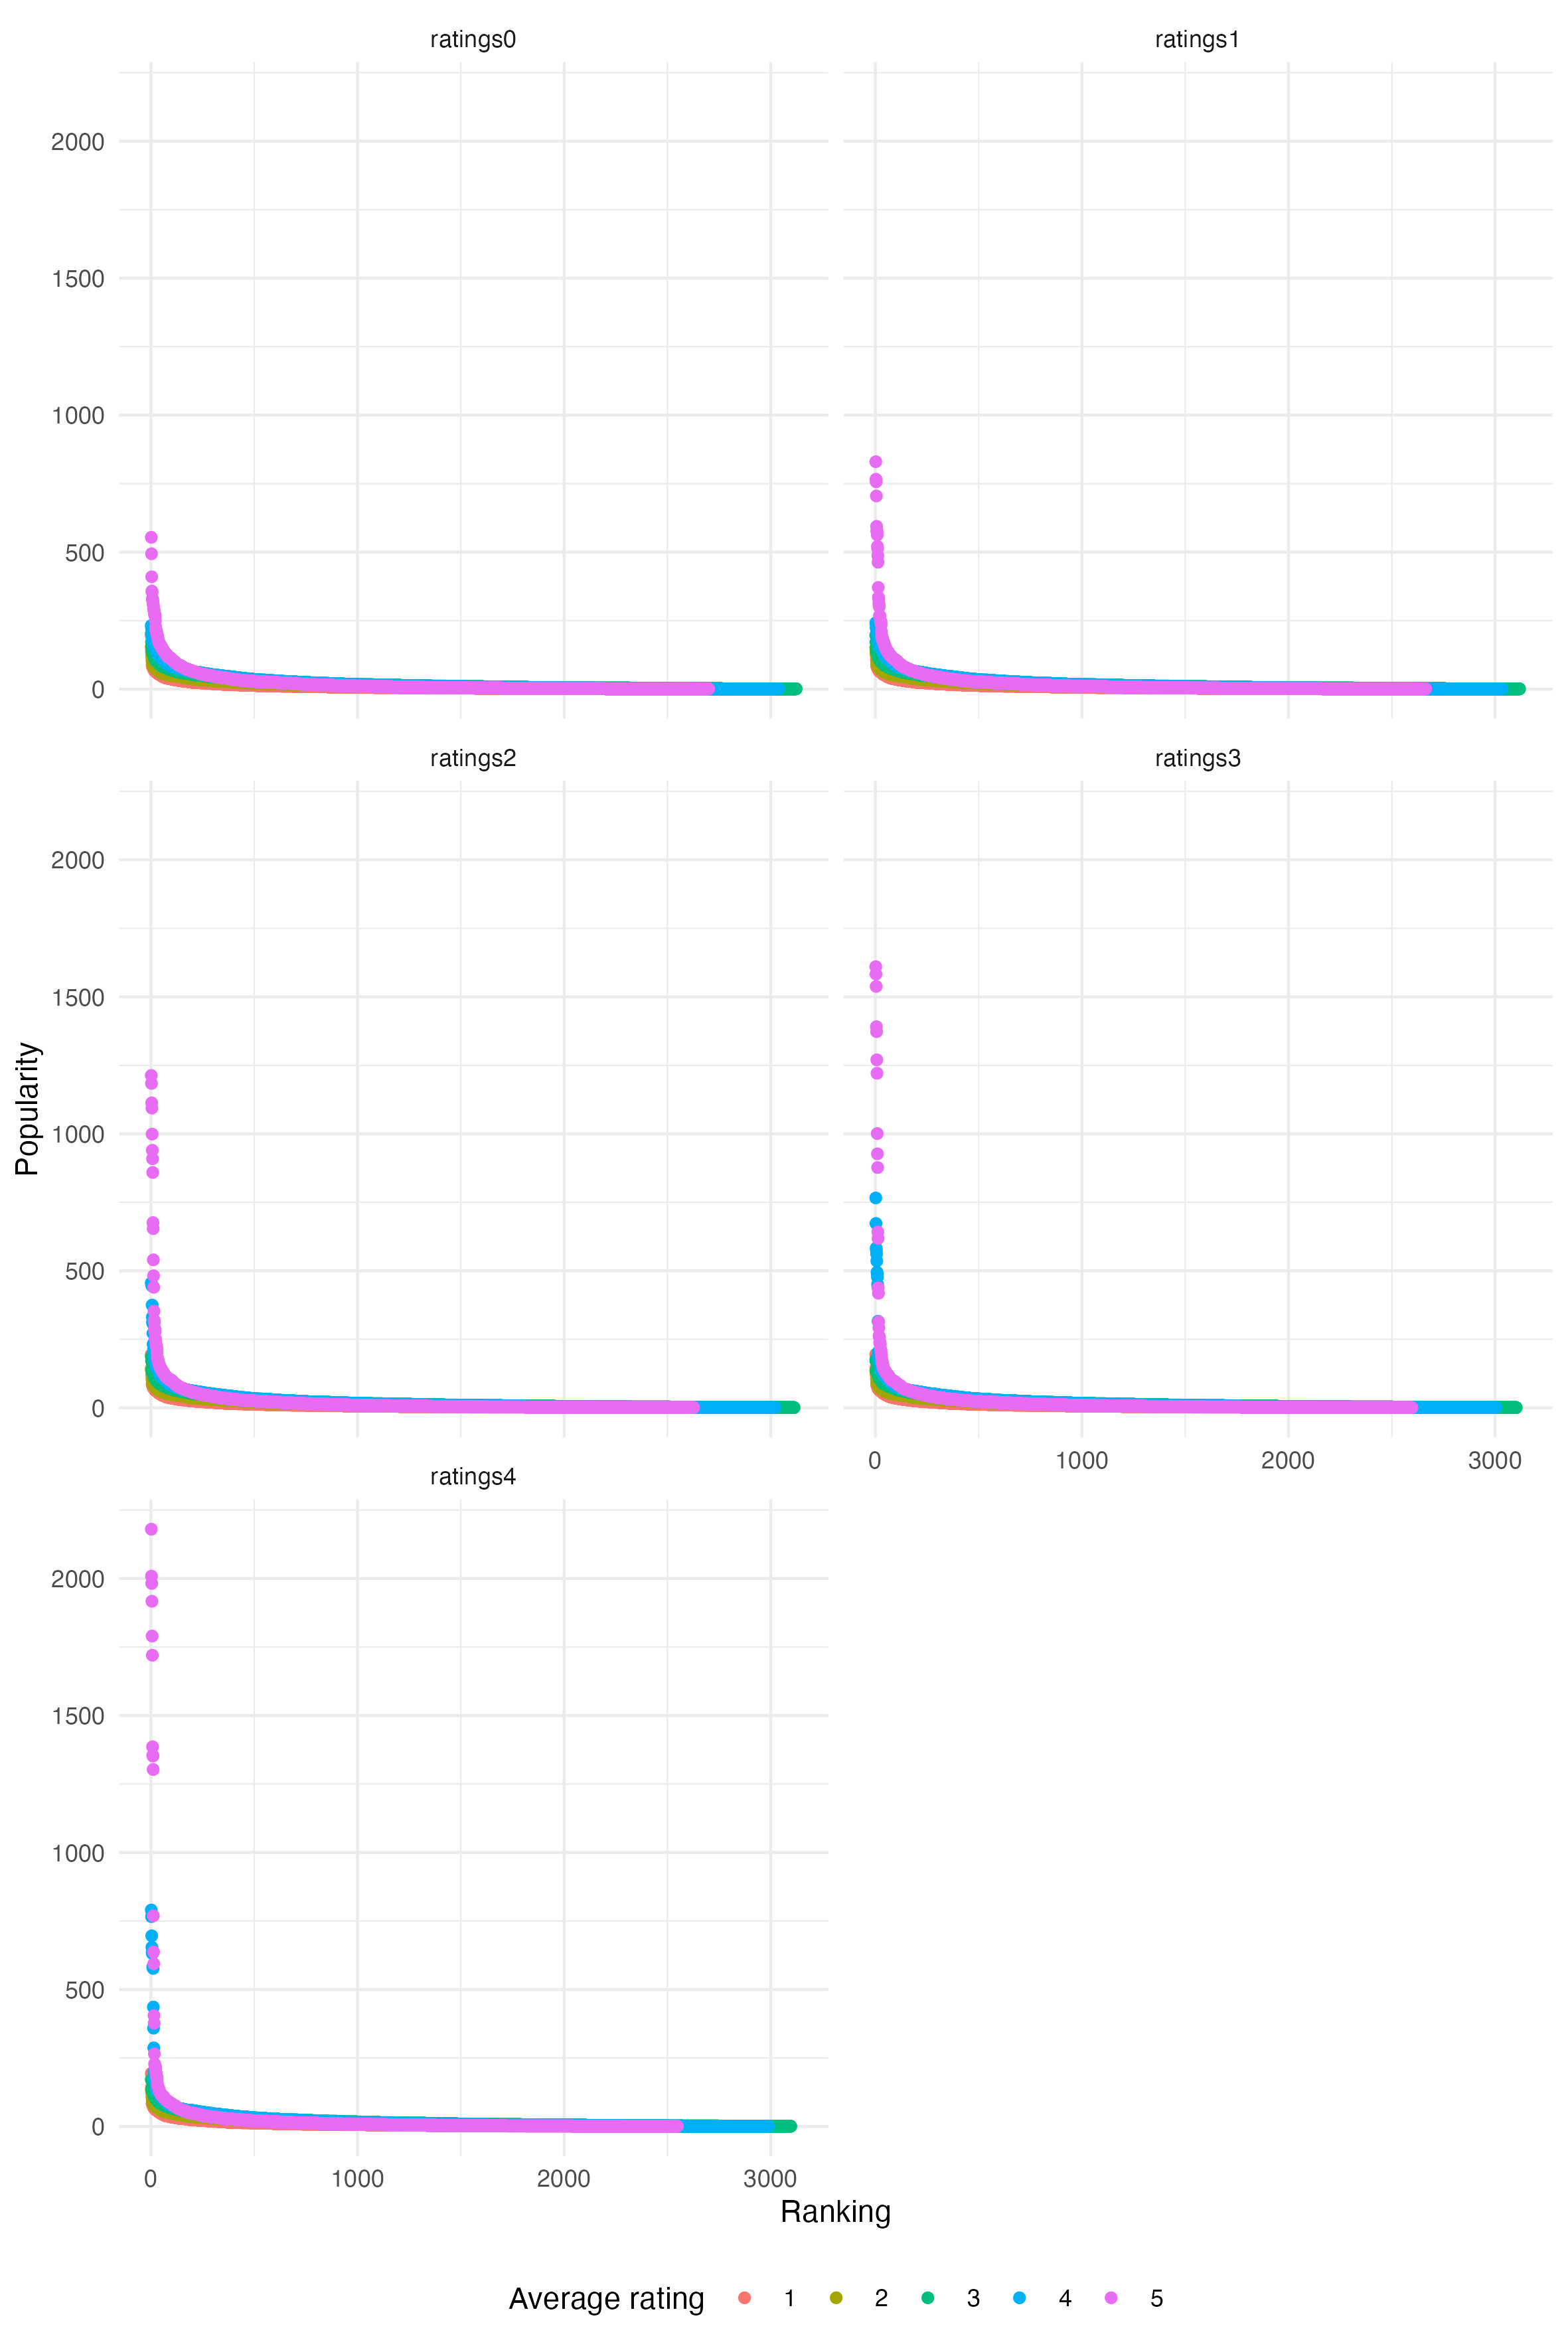
\includegraphics[width=\textwidth]{04_profile_grouped}
  \caption{Recommendation profile of every generation. Colors indicate average
  movie rating, which is a strong predictor of popularity over time.
  \label{fig:fig04_profile_grouped}}
\end{figure}

% explicar que, nos gráficos, popularidade significa número de recs para t = 1..4

A good way to measure how diverse were the recommendations made by the algorithm
is to calculate the entropy \citep{} of each set. In the extreme, if the same
movie is recommended to every user, than the entropy of the recommendations will
tend to zero. In absolute terms, the entropy of \verb|ratings0| was 7.42, and
the entropy of \verb|ratings4| was 6.08 (82\% lower). A comparison in relative
terms is displayed in Figure~\ref{fig:fig04_entropy}.

\begin{figure}
  \centering
  \begin{subfigure}{0.45\textwidth}
    \centering
    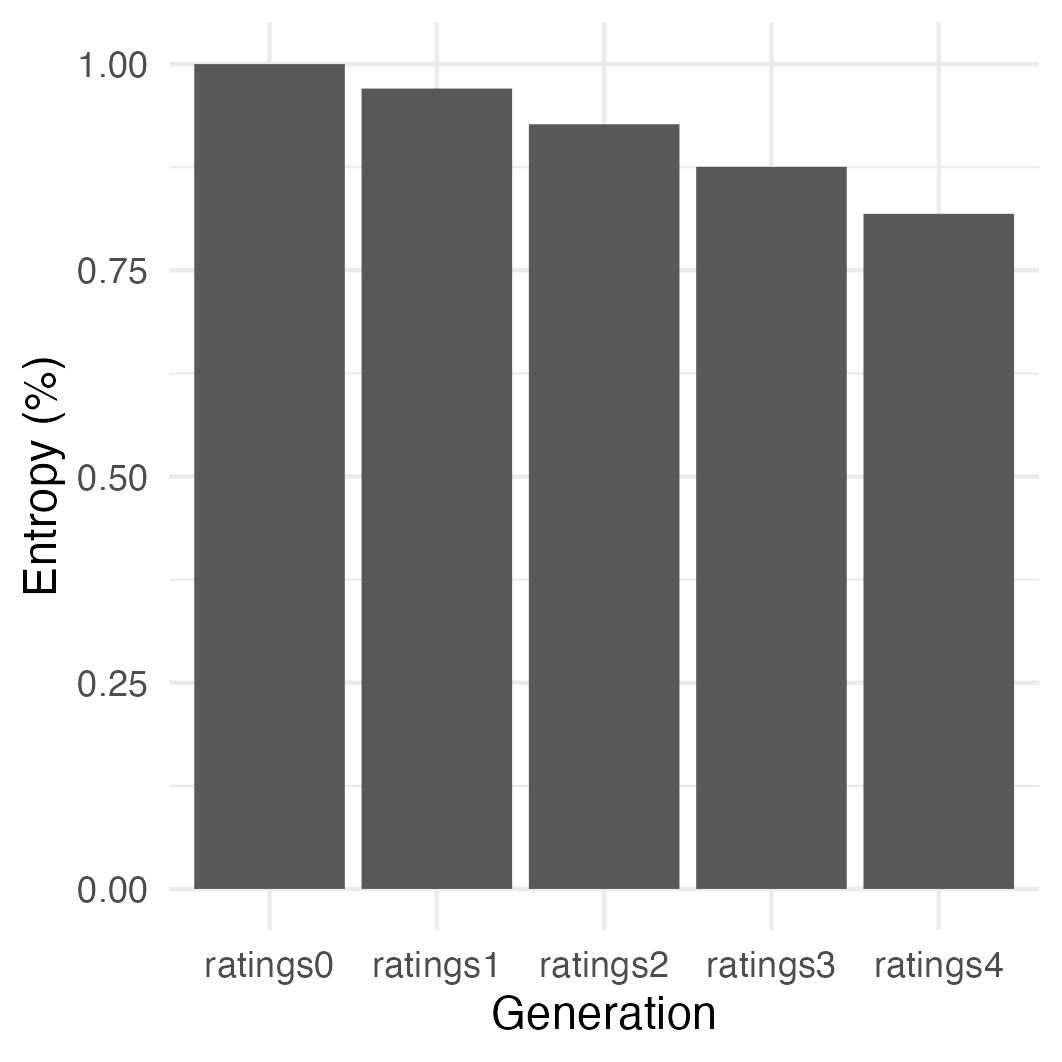
\includegraphics[width=\textwidth]{04_entropy}
  \end{subfigure}
  \caption{Recommendation entropy as a percentage of ratings0s entropy.
  \label{fig:fig04_entropy}}
\end{figure}

We can also observe this reduction of variety in an even more visual way. In
Figure~\ref{fig:fig04_popularity_time_both} we plotted movie popularity over
time; each line represents a movie and each step in the x-axis is a new
generation of the model. Figure~\ref{fig:fig04_popularity_time} makes it very
clear that no more than 15 movies rose in popularity over the four generations
of the recommendation system, becoming orders of magnitude more popular than the
rest. We also scaled the y-axis by taking the its log in
Figure~\ref{fig:fig04_log_popularity_time}, and we can see that, in fact, no
other movie rose in popularity besides the ones that stick out after
\verb|model2|.

It is also of note that the few movies that rise in popularity are not the most
popular ones from \verb|ratings0|, even though genre was the only metadata we
fed into the system. This uncovers a significant feature of the feedback loop we
observed in Figure~\ref{fig:fig04_profile_grouped}: the items that the algorithm
amplifies don't necessarily have to be the most mainstream, or in other words,
recommendation systems are able to boost content artificially.

\begin{figure}
  \centering
  \begin{subfigure}{0.45\textwidth}
    \centering
    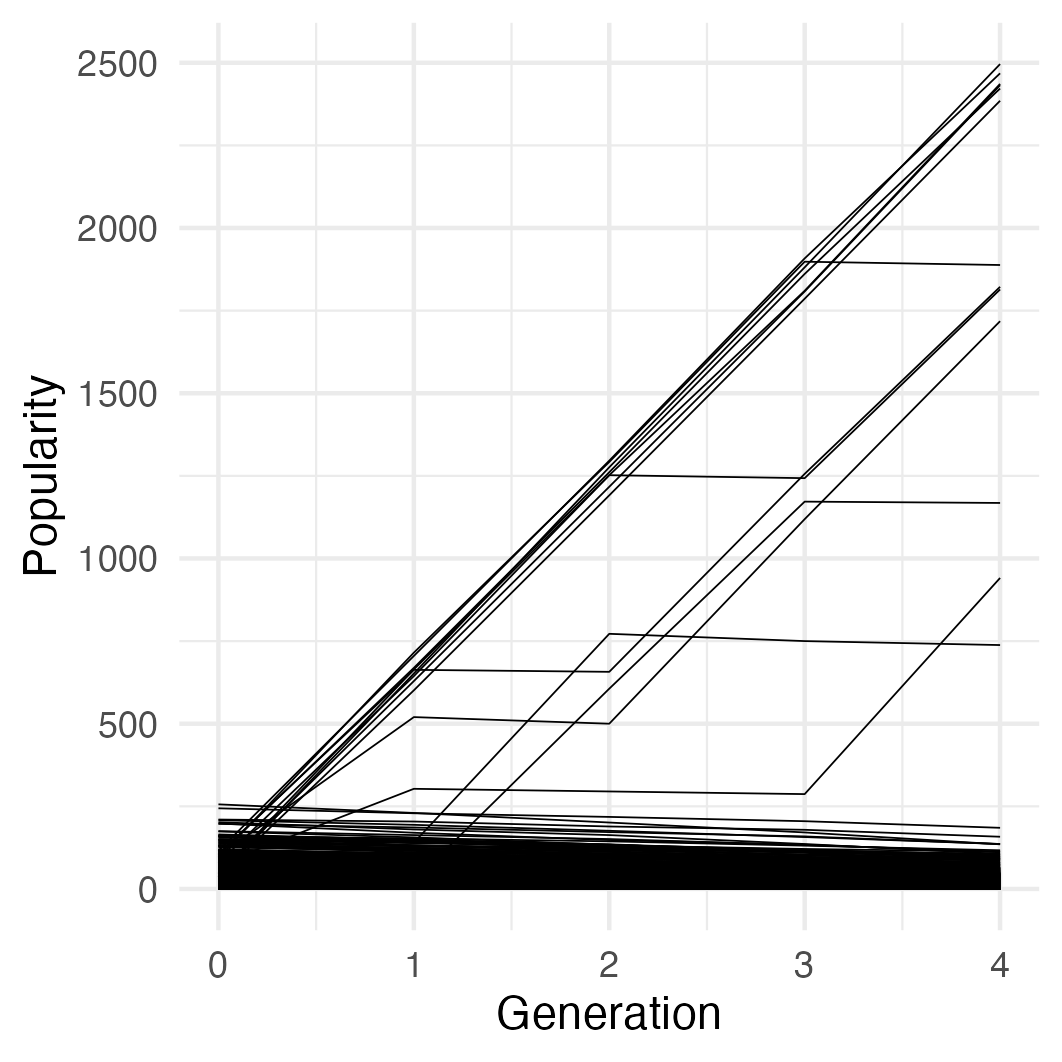
\includegraphics[width=\textwidth]{04_popularity_time}
    \caption{Movie popularity over time.\label{fig:fig04_popularity_time}}
  \end{subfigure}
  \begin{subfigure}{0.45\textwidth}
    \centering
    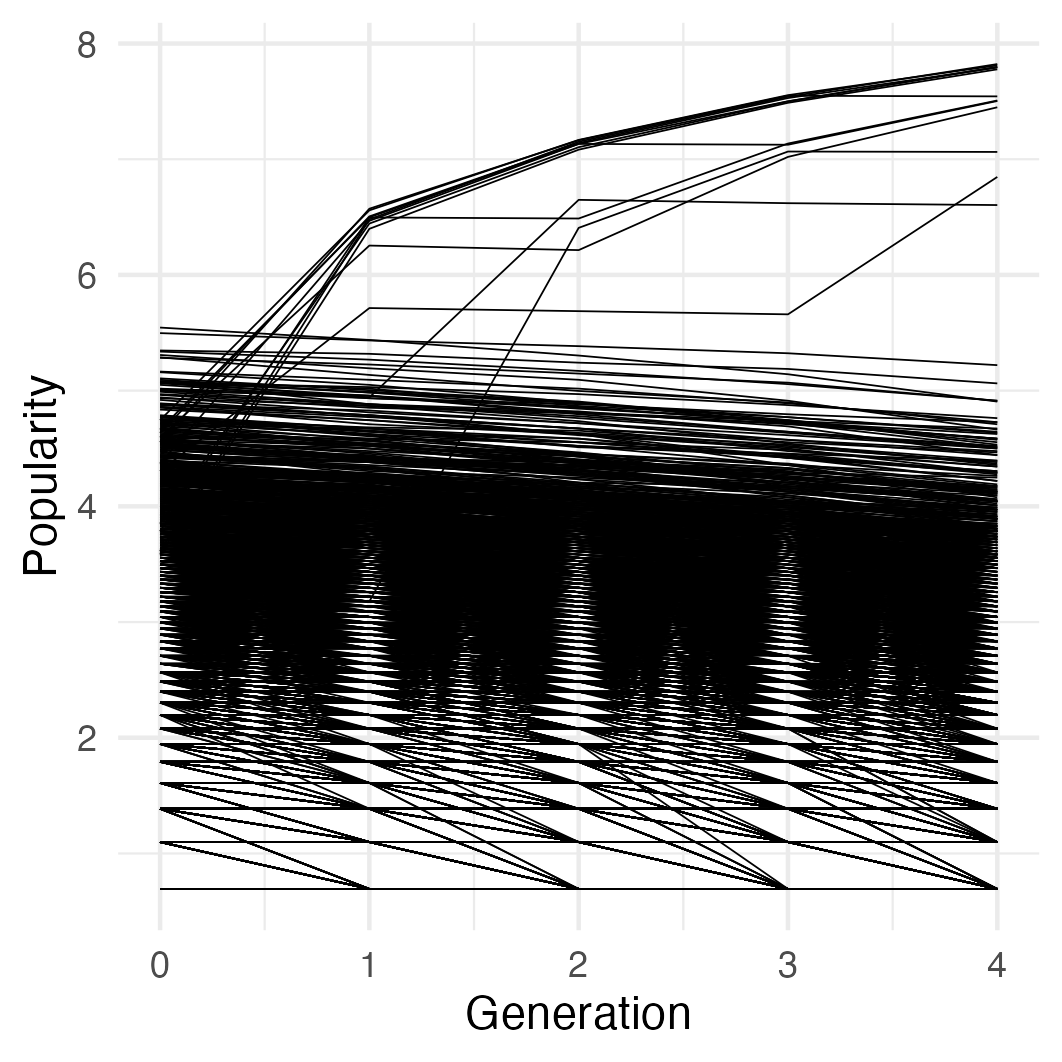
\includegraphics[width=\textwidth]{04_log_popularity_time}
    \caption{Movie log-popularity over time.\label{fig:fig04_log_popularity_time}}
  \end{subfigure}
  \caption{Popularity of every movie from ratings0 to ratings4.\label{fig:fig04_popularity_time_both}}
\end{figure}

\section{Modeling}
\label{sec:modeling04}

Having identified a feedback loop in the recommendation system, we decided to
fit a regression model on our generated data. The goal of this step is
essentially explainability \citep{}: to help better understand the algorithms
decisions.

% Computational Statistics do James E. Gentle

As is common in computational inference \citep{}, our process involved multiple
rounds of modeling. We started with a very simple model and, according to
goodness-of-fit measurements, made it more and more complex in order to achieve
a better representation of the behavior of the recommendation system. As we will
see later, even after feeding all of the the available data (and some extra
metadata that the recommender algorithm didn't have access to), our models were
not able to capture such a degenerate distribution.

The first model we attempted to use was a simple Poisson regression \citep{}.
Since the recommendation profiles displayed a strong positive skew and an
exponential-like decay, a log-linear model seemed like a good starting point.
For this kind of model \citep{}, we take a set of $\mathbf{x} \in
\mathbb{R}^{n}$ and fit a regression of the form

$$
\log(\operatorname{E} (Y \mid \mathbf{x})) = \alpha + \mathbf{\beta}'\mathbf{x},
$$

where $\alpha \in \mathbb{R}$ and $\mathbf{\beta} \in \mathbb{R}^{n}$. More
concretely, we used R's \verb|glm()| \citep{} function with the following
formula: \verb|pop ~ t * genre * rating|. In this expression, \verb|pop|
represents the popularity of a movie, \verb|t| represents the generation i.e.
the iteration from 0 to 4, and \verb|genre| represents the genre.

As the reader might be able to see, we used the genre variable in our regression
model even though we didn't feed it to the recommendation system. As explained
before, the algorithm only had access to the popularity and ratings of the
movies, but it is possible the there exists a latent effect of genre on the
other variables; since a machine learning system is much more flexible than a
regression model, we opted to explicitly feed the genre into the Poisson model
and all others that followed.

For illustrative purposes, we will present the full output of this model below.
It is notable how many coefficients are considered highly significant, meaning
that, individually, they were able to capture the feedback loop generated by
the recommendation system.

\begin{verbatim}
Call:
glm(formula = pop ~ t * genre * rating, family = "poisson", data = features)

Deviance Residuals:
    Min       1Q   Median       3Q      Max
-33.145   -3.088   -1.222    1.260   93.001

Coefficients:
                            Estimate Std. Error z value Pr(>|z|)
(Intercept)                9.210e-02  9.514e-02   0.968 0.333031
t                         -6.844e-02  4.200e-02  -1.629 0.103208
genreAnimation            -2.276e+00  1.475e-01 -15.430  < 2e-16 ***
genreChildren's            1.489e-02  1.754e-01   0.085 0.932347
genreComedy               -1.904e-01  1.041e-01  -1.828 0.067539 .
genreCrime                -4.898e+00  1.858e-01 -26.364  < 2e-16 ***
genreDocumentary          -1.801e+00  4.491e-01  -4.010 6.07e-05 ***
genreDrama                -1.035e+00  1.140e-01  -9.086  < 2e-16 ***
genreFilm-Noir            -1.631e+01  5.403e-01 -30.185  < 2e-16 ***
genreHorror                3.012e-01  1.178e-01   2.556 0.010582 *
genreMusical              -2.784e+00  4.813e-01  -5.784 7.31e-09 ***
genreMystery              -4.849e+00  2.464e-01 -19.681  < 2e-16 ***
genreRomance              -1.476e+00  5.299e-01  -2.785 0.005347 **
genreSci-Fi                1.583e+00  1.898e-01   8.341  < 2e-16 ***
genreThriller              3.854e-01  1.791e-01   2.152 0.031394 *
genreWestern              -4.253e+00  5.017e-01  -8.476  < 2e-16 ***
rating                     8.877e-01  2.740e-02  32.395  < 2e-16 ***
t:genreAnimation          -3.139e+00  6.223e-02 -50.435  < 2e-16 ***
t:genreChildren's         -5.212e-04  7.760e-02  -0.007 0.994641
t:genreComedy             -2.235e-02  4.602e-02  -0.486 0.627215
t:genreCrime              -3.561e+00  8.570e-02 -41.557  < 2e-16 ***
t:genreDocumentary         2.463e-01  1.933e-01   1.274 0.202583
t:genreDrama              -1.845e+00  5.015e-02 -36.799  < 2e-16 ***
t:genreFilm-Noir          -5.419e+00  1.944e-01 -27.872  < 2e-16 ***
t:genreHorror              7.776e-03  5.217e-02   0.149 0.881511
t:genreMusical             1.190e-01  2.140e-01   0.556 0.578236
t:genreMystery            -3.676e+00  1.032e-01 -35.632  < 2e-16 ***
t:genreRomance            -8.909e-02  2.334e-01  -0.382 0.702658
t:genreSci-Fi             -2.251e+00  8.076e-02 -27.869  < 2e-16 ***
t:genreThriller            6.362e-02  7.894e-02   0.806 0.420240
t:genreWestern             5.290e-02  2.211e-01   0.239 0.810874
t:rating                  -1.584e-02  1.212e-02  -1.307 0.191193
genreAnimation:rating      7.049e-01  3.938e-02  17.900  < 2e-16 ***
genreChildren's:rating    -4.814e-02  5.303e-02  -0.908 0.364006
genreComedy:rating         1.711e-02  2.989e-02   0.572 0.567055
genreCrime:rating          1.261e+00  4.818e-02  26.161  < 2e-16 ***
genreDocumentary:rating    5.638e-02  1.160e-01   0.486 0.626776
genreDrama:rating          1.163e-01  3.199e-02   3.635 0.000278 ***
genreFilm-Noir:rating      3.865e+00  1.239e-01  31.197  < 2e-16 ***
genreHorror:rating        -1.456e-01  3.541e-02  -4.111 3.95e-05 ***
genreMusical:rating        6.395e-01  1.255e-01   5.095 3.50e-07 ***
genreMystery:rating        1.286e+00  6.114e-02  21.030  < 2e-16 ***
genreRomance:rating        3.492e-02  1.506e-01   0.232 0.816639
genreSci-Fi:rating        -5.037e-01  5.457e-02  -9.230  < 2e-16 ***
genreThriller:rating      -1.952e-01  5.094e-02  -3.833 0.000127 ***
genreWestern:rating        9.773e-01  1.309e-01   7.467 8.19e-14 ***
t:genreAnimation:rating    8.263e-01  1.631e-02  50.671  < 2e-16 ***
t:genreChildren's:rating  -1.370e-03  2.350e-02  -0.058 0.953503
t:genreComedy:rating       6.194e-03  1.323e-02   0.468 0.639610
t:genreCrime:rating        9.129e-01  2.163e-02  42.204  < 2e-16 ***
t:genreDocumentary:rating -5.843e-02  5.002e-02  -1.168 0.242813
t:genreDrama:rating        5.028e-01  1.399e-02  35.927  < 2e-16 ***
t:genreFilm-Noir:rating    1.279e+00  4.402e-02  29.061  < 2e-16 ***
t:genreHorror:rating      -6.526e-03  1.573e-02  -0.415 0.678237
t:genreMusical:rating     -3.530e-02  5.588e-02  -0.632 0.527603
t:genreMystery:rating      9.553e-01  2.495e-02  38.291  < 2e-16 ***
t:genreRomance:rating      3.023e-02  6.624e-02   0.456 0.648140
t:genreSci-Fi:rating       6.707e-01  2.195e-02  30.551  < 2e-16 ***
t:genreThriller:rating    -1.870e-02  2.252e-02  -0.830 0.406351
t:genreWestern:rating     -1.209e-02  5.768e-02  -0.210 0.834031
---
Signif. codes:  0 ‘***’ 0.001 ‘**’ 0.01 ‘*’ 0.05 ‘.’ 0.1 ‘ ’ 1

(Dispersion parameter for poisson family taken to be 1)

    Null deviance: 562028  on 13559  degrees of freedom
Residual deviance: 268737  on 13500  degrees of freedom
AIC: 318813

Number of Fisher Scoring iterations: 6
\end{verbatim}

However, analyzing the coefficients by themselves is only one part of the full
picture. We used a simulation envelope \citep{} to assess global
goodness-of-fit, which is obtained by plotting the ordered absolute values of a
model diagnostic versus the expected order statistic of a normal distribution
\citep{}:

$$
\Phi^{-1}(\frac{i+3/8}{n+1/4})
$$

% Reescrever os 2 parágrafos abaixo. Eles foram tirados direto dos docs da
% hnp::hnp()

% Atkinson (1985)
\citet{} proposed the addition of a simulated envelope, which is such that under
the correct model the plot for the observed data is likely to fall within the
envelope. The objective is not to provide a region of acceptance, but some sort
of guidance to what kind of shape to expect.

Obtaining the simulated envelope is simple and consists of (1) fitting a model;
(2) extracting model diagnostics and calculating sorted absolute values; (3)
simulating 99 (or more) response variables using the same model matrix, error
distribution and fitted parameters; (4) fitting the same model to each simulated
response variable and obtaining the same model diagnostics, again sorted
absolute values; (5) computing the desired percentiles (e.g., 2.5 and 97.5) at
each value of the expected order statistic to form the envelope.

The resulting simulated envelope was generated with the \verb|hnp| \citep{} R
package and can be seen in Figure~\ref{fig:fig04_residual_poisson}. It is plain
to see that the model does not conform to the delimited region and, therefore,
isn't able to properly capture the variability of the data.

\begin{figure}
  \centering
  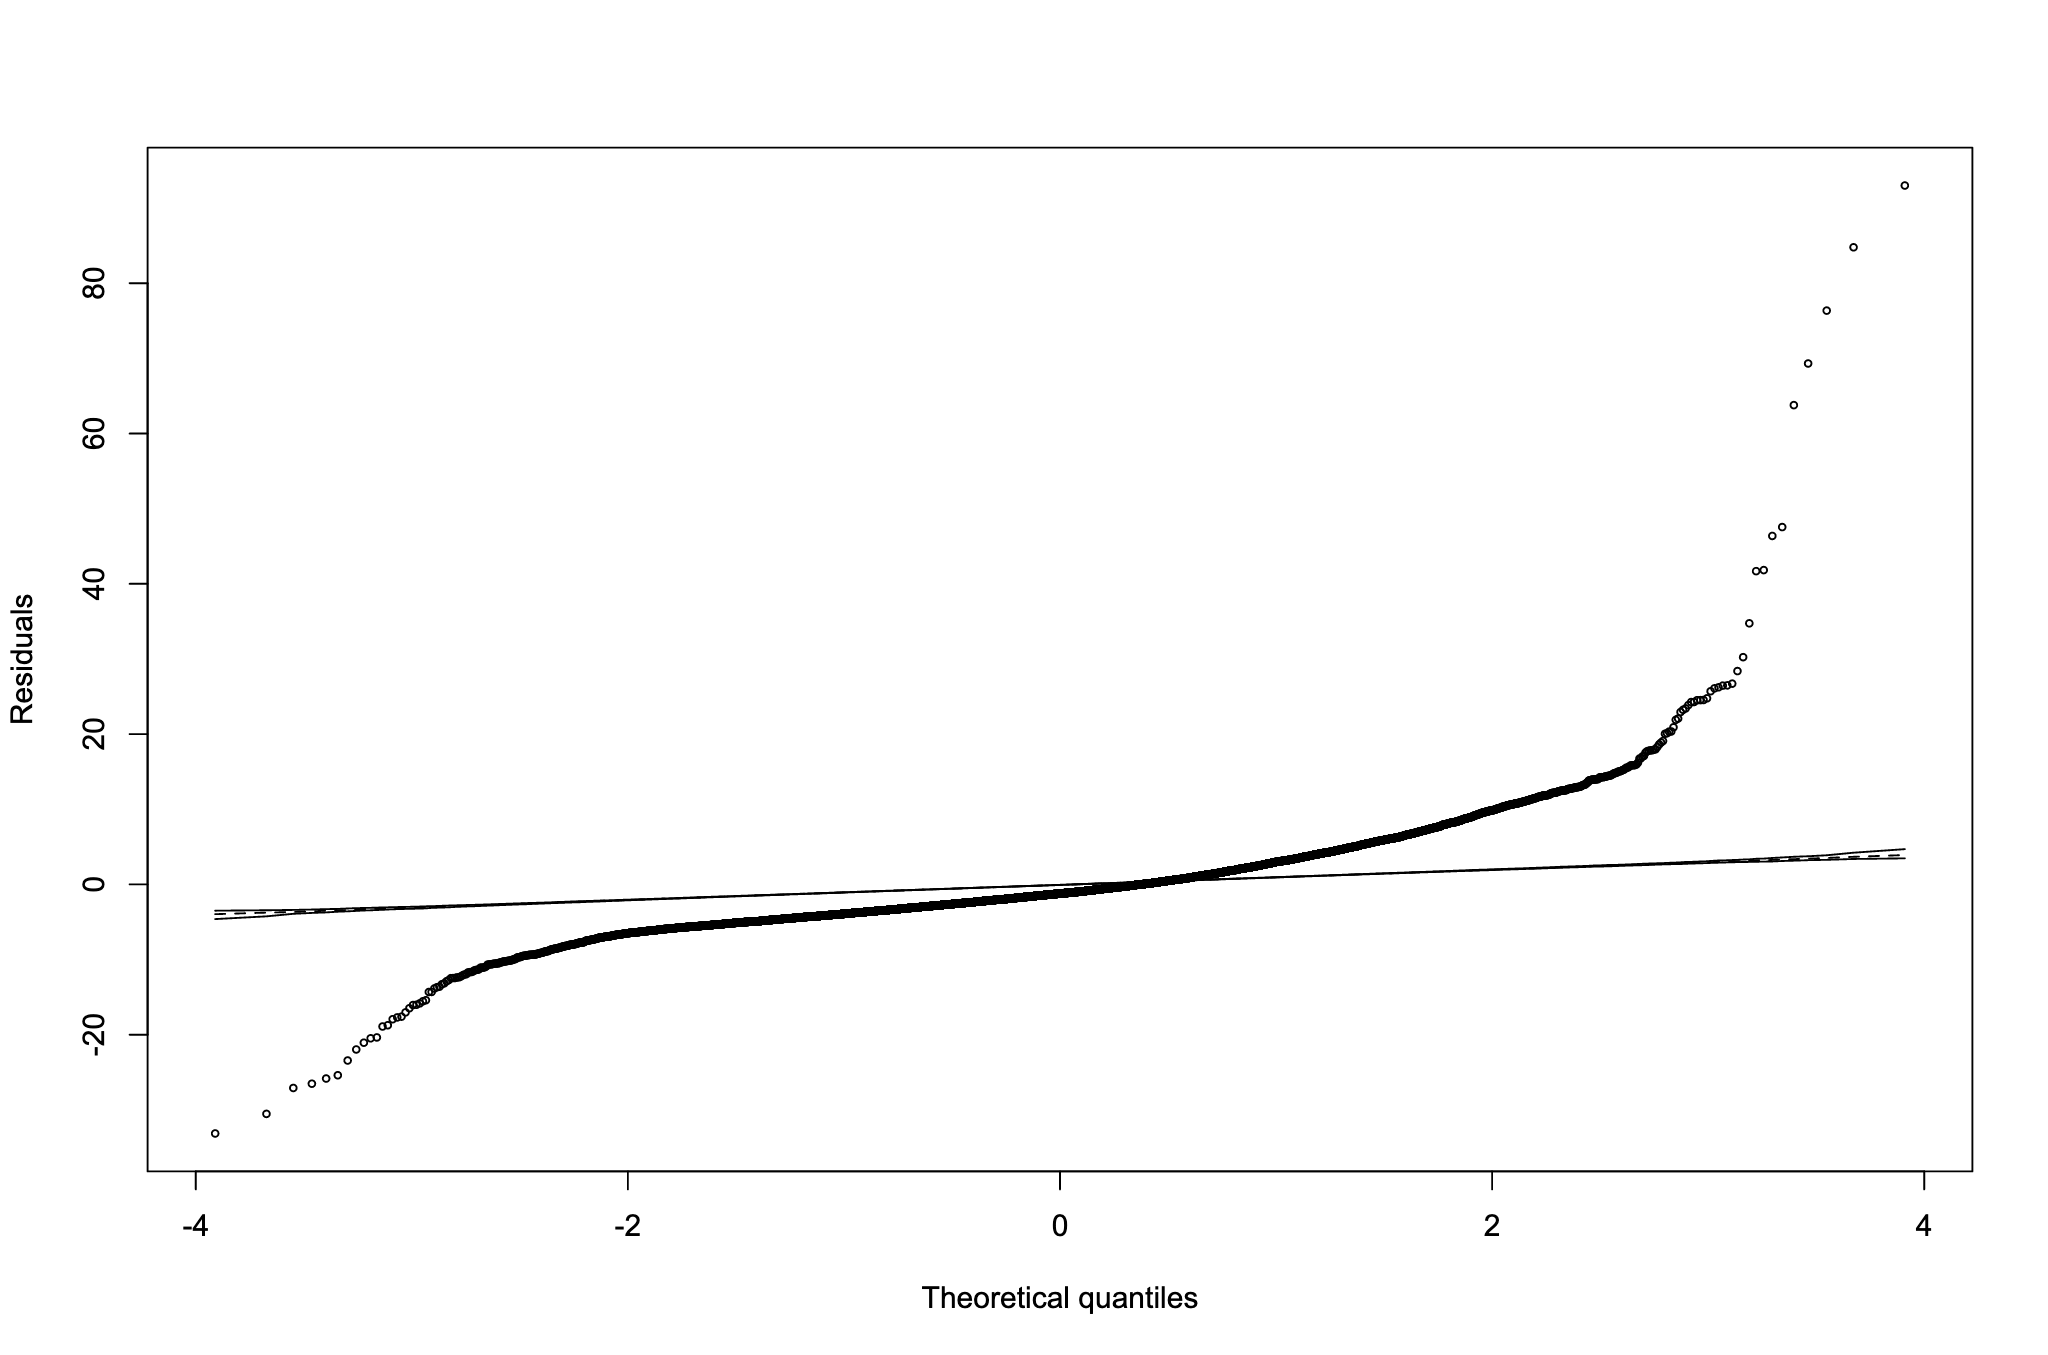
\includegraphics[width=\textwidth]{04_residual_poisson}
  \caption{Residual analysis via simulated envelope for the Poisson regression.\label{fig:fig04_residual_poisson}}
\end{figure}




..., and \verb|movie_id| is the ID of a movie. Note
that the genre was not used when training the recommendation models described
above, but it turned out that this feature could explain a lot of the models'
outputs.

\begin{verbatim}
  Family: nbinom2  ( log )
Formula:          pop ~ t * genre * rating + (1 | movie_id)
Data: features

     AIC      BIC   logLik deviance df.resid
 83863.8  84370.3 -41865.9  83731.8    15844

Random effects:

Conditional model:
 Groups   Name        Variance Std.Dev.
 movie_id (Intercept) 1.364    1.168
Number of obs: 15910, groups:  movie_id, 3182

Dispersion parameter for nbinom2 family ():   49

Conditional model:
                            Estimate Std. Error z value Pr(>|z|)
(Intercept)                -0.108714   0.272464  -0.399 0.689891
t                          -0.210272   0.021153  -9.941  < 2e-16 ***
genreAdventure              0.112129   0.574197   0.195 0.845174
genreAnimation             -2.286362   0.773873  -2.954 0.003132 **
genreChildren's             0.855196   0.755919   1.131 0.257915
genreComedy                -0.108159   0.352431  -0.307 0.758925
genreCrime                 -3.590470   0.850227  -4.223 2.41e-05 ***
genreDocumentary           -1.659325   1.508329  -1.100 0.271285
genreDrama                 -1.219969   0.409312  -2.981 0.002877 **
genreFilm-Noir            -16.633103   2.371128  -7.015 2.30e-12 ***
genreHorror                 0.512807   0.443025   1.158 0.247062
genreMusical               -4.259252   2.088483  -2.039 0.041410 *
genreMystery               -4.646920   1.461852  -3.179 0.001479 **
genreRomance               -2.118789   1.856289  -1.141 0.253699
genreSci-Fi                 0.363380   1.044431   0.348 0.727899
genreThriller               1.382908   0.855392   1.617 0.105944
genreWestern               -3.766758   2.108848  -1.786 0.074072 .
rating                      0.957533   0.085468  11.203  < 2e-16 ***
t:genreAdventure            0.161327   0.053403   3.021 0.002520 **
t:genreAnimation           -0.392012   0.067698  -5.791 7.01e-09 ***
t:genreChildren's           0.116028   0.066946   1.733 0.083068 .
t:genreComedy               0.119502   0.030504   3.918 8.94e-05 ***
t:genreCrime               -0.146821   0.085503  -1.717 0.085952 .
t:genreDocumentary          0.329357   0.195776   1.682 0.092507 .
t:genreDrama                0.005393   0.038739   0.139 0.889287
t:genreFilm-Noir           -0.730742   0.227275  -3.215 0.001303 **
t:genreHorror               0.148203   0.041813   3.544 0.000393 ***
t:genreMusical              0.265118   0.243060   1.091 0.275383
t:genreMystery             -1.150785   0.123034  -9.353  < 2e-16 ***
t:genreRomance              0.064921   0.227735   0.285 0.775590
t:genreSci-Fi              -0.311108   0.079779  -3.900 9.63e-05 ***
t:genreThriller             0.134758   0.077077   1.748 0.080403 .
t:genreWestern              0.184582   0.216581   0.852 0.394073
t:rating                    0.029594   0.006273   4.717 2.39e-06 ***
genreAdventure:rating      -0.209253   0.179840  -1.164 0.244606
genreAnimation:rating       0.594327   0.226301   2.626 0.008633 **
genreChildren's:rating     -0.473591   0.247951  -1.910 0.056131 .
genreComedy:rating         -0.194909   0.109223  -1.785 0.074341 .
genreCrime:rating           0.736375   0.243050   3.030 0.002448 **
genreDocumentary:rating    -0.113489   0.399299  -0.284 0.776242
genreDrama:rating          -0.031020   0.120957  -0.256 0.797601
genreFilm-Noir:rating       3.958891   0.595316   6.650 2.93e-11 ***
genreHorror:rating         -0.422452   0.151685  -2.785 0.005352 **
genreMusical:rating         0.944897   0.569196   1.660 0.096903 .
genreMystery:rating         1.092607   0.409047   2.671 0.007560 **
genreRomance:rating         0.013712   0.548422   0.025 0.980053
genreSci-Fi:rating         -0.423339   0.324094  -1.306 0.191477
genreThriller:rating       -0.729129   0.256016  -2.848 0.004400 **
genreWestern:rating         0.725673   0.578412   1.255 0.209625
t:genreAdventure:rating    -0.053250   0.015828  -3.364 0.000768 ***
t:genreAnimation:rating     0.110189   0.018603   5.923 3.16e-09 ***
t:genreChildren's:rating   -0.039499   0.020922  -1.888 0.059031 .
t:genreComedy:rating       -0.039790   0.008913  -4.464 8.04e-06 ***
t:genreCrime:rating         0.038460   0.022654   1.698 0.089557 .
t:genreDocumentary:rating  -0.088874   0.050610  -1.756 0.079076 .
t:genreDrama:rating        -0.006800   0.010754  -0.632 0.527202
t:genreFilm-Noir:rating     0.183567   0.054187   3.388 0.000705 ***
t:genreHorror:rating       -0.052874   0.013574  -3.895 9.81e-05 ***
t:genreMusical:rating      -0.082105   0.063538  -1.292 0.196285
t:genreMystery:rating       0.335177   0.032553  10.296  < 2e-16 ***
t:genreRomance:rating      -0.018634   0.064877  -0.287 0.773939
t:genreSci-Fi:rating        0.108210   0.023442   4.616 3.91e-06 ***
t:genreThriller:rating     -0.044310   0.022584  -1.962 0.049758 *
t:genreWestern:rating      -0.055461   0.056878  -0.975 0.329521
---
Signif. codes:  0 '***' 0.001 '**' 0.01 '*' 0.05 '.' 0.1 ' ' 1
\end{verbatim}

\begin{figure}
  \centering
  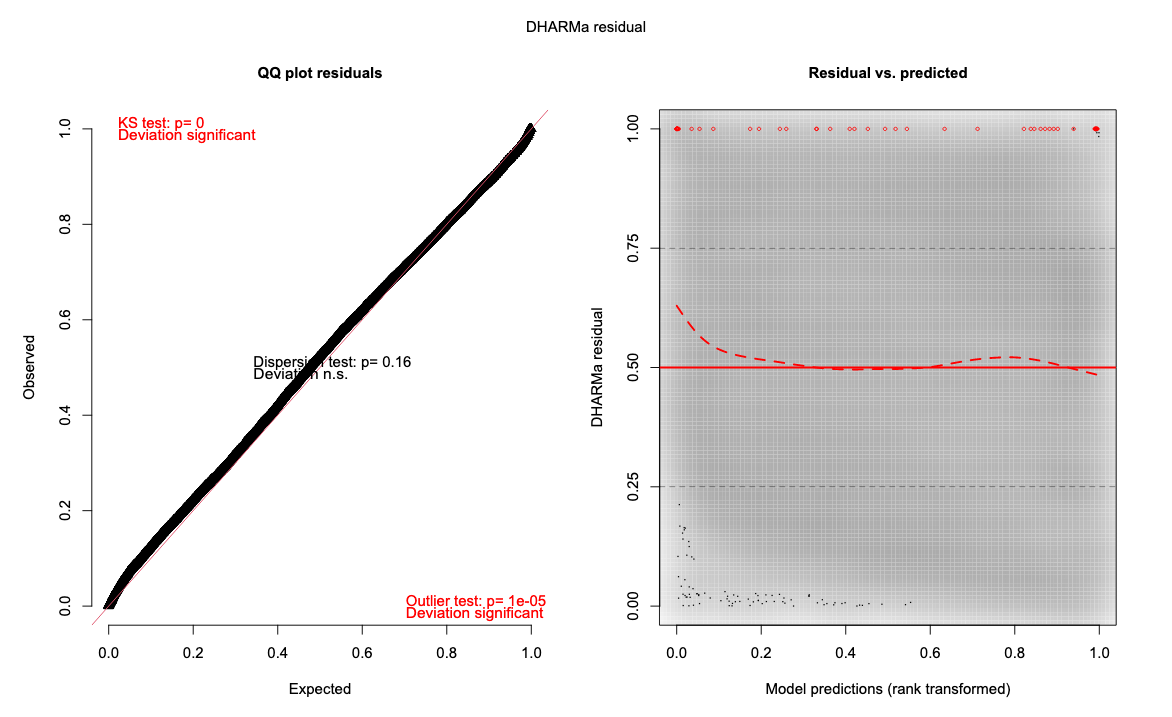
\includegraphics[width=\textwidth]{04_residual_mmnb2}
  \caption{Residual analysis for glmmTMB model.\label{fig:fig04_residual_mmnb2}}
\end{figure}

\par
